% !TeX encoding = UTF-8
% !TeX program = xelatex
% !TeX spellcheck = en_US

\documentclass[]{shcmthesis}
  % 字体库 fontset
  %   windows | mac | fandol | ubuntu
  % 建议终版使用 Windows 平台的字体编译


% 论文基本配置,加载宏包等全局配置
% !TeX root = ./shcmthesis-example.tex

% 论文基本信息配置

\thusetup{
  %******************************
  % 注意:
  %   1. 配置里面不要出现空行
  %   2. 不需要的配置信息可以删除
  %   3. 建议先阅读文档中所有关于选项的说明
  %******************************
  %
  % 输出格式
  %   选择打印版(print)或用于提交的电子版(electronic),前者会插入空白页以便直接双面打印
  %
  output = electronic,
  %
  %
  % 封面格式
  %	  选择用于预审(preliminary)或用于最终提交的终版(final)
  %
  cover = final,
  %
  %
  % 学位类型
  %   选择本科(bachelor)、硕士(master)或者博士(doctor)
  %
  degree = doctor,
  %
  %
  % 论文标题
  %   -1和-2分别对应标题的第一行和第二行,加*的为英文标题
  %
  title-1  = {上海音乐学院学位论文},
  title-2  = {\LaTeX{} 模板 v\version},
  title-1* = {\LaTeX{} v\version~Thesis Template},
  title-2* = {Shanghai Conservatory of Music},
  %  
  %  
  % 论文编号
  %
  thesis-id = {001},
  % 
  % 
  % 学校代码
  % 
  school-id = {10278},
  %
  %
  % 学科专业
  %
  discipline  = {音乐与舞蹈学/中国音乐研究},
  %
  % 研究方向
  %
  professional-field  = {中国传统音乐理论},
  %
  % 作者姓名
  %
  author  = {王丹丹},
  %
  % 作者学号
  %
  student-id = {D202000},
  %
  % 指导教师
  %   中文姓名和职称之间以\quad分开
  %
  supervisor  = {李红\quad 教授},
  %
  % 完成日期
  %
  date = {2025年6月},
  %
  % 是否在中文封面后的空白页生成书脊(默认 false)
  %
  include-spine = false,
  %
}

% 载入所需的宏包

% 定理类环境宏包
\usepackage{amsthm}
% 也可以使用 ntheorem
% \usepackage[amsmath,thmmarks,hyperref]{ntheorem}

\thusetup{
  %
  % 数学字体
  % math-style = GB,  % GB | ISO | TeX
  math-font  = xits,  % stix | xits | libertinus
}

% 可以使用 nomencl 生成符号和缩略语说明
% \usepackage{nomencl}
% \makenomenclature

% 表格加脚注
\usepackage{threeparttable}

% 表格中支持跨行
\usepackage{multirow}

% 固定宽度的表格。
% \usepackage{tabularx}

% 跨页表格
\usepackage{longtable}

% 算法
\usepackage{algorithm}
\usepackage{algorithmic}

% 代码块
\usepackage{pythonhighlight}

% 量和单位
\usepackage{siunitx}

% 参考文献使用 BibTeX + natbib 宏包
% 顺序编码制
% \usepackage[sort]{natbib}

% 参考文献使用 BibLaTeX 宏包
% \usepackage[style=gb7714-2015]{biblatex}
% 声明 BibLaTeX 的数据库
% \addbibresource{ref/refs.bib}

% 定义所有的图片文件在 figures 子目录下
\graphicspath{{figures/}}

% 数学命令
\makeatletter
\newcommand\dif{%  % 微分符号
  \mathop{}\!%
  \ifthu@math@style@TeX
    d%
  \else
    \mathrm{d}%
  \fi
}
\makeatother

% hyperref 宏包在最后调用
\usepackage{hyperref}



\begin{document}

% 封面
\maketitle

% 学位论文指导小组、公开评阅人和答辩委员会名单
% \input{data/committee}

% 使用授权的说明
\copyrightpage
% 将签字扫描后授权文件 scan-copyright.pdf 替换原始页面
% \copyrightpage[file=scan-copyright.pdf]

\frontmatter
% !TeX root = ../shcmthesis-example.tex

% 中英文摘要和关键字

\begin{abstract}
  论文的摘要是对论文研究内容和成果的高度概括。
  摘要应对论文所研究的问题及其研究目的进行描述,对研究方法和过程进行简单介绍,对研究成果和所得结论进行概括。
  摘要应具有独立性和自明性,其内容应包含与论文全文同等量的主要信息。
  使读者即使不阅读全文,通过摘要就能了解论文的总体内容和主要成果。

  论文摘要的书写应力求精确、简明。
  切忌写成对论文书写内容进行提要的形式,尤其要避免“第 1 章……;第 2 章……;……”这种或类似的陈述方式。

  关键词是为了文献标引工作、用以表示全文主要内容信息的单词或术语。
  关键词不超过 5 个,每个关键词中间用分号分隔。

  % 关键词用“英文逗号”分隔,输出时会自动处理为正确的分隔符
  \thusetup{
    keywords = {关键词 1, 关键词 2, 关键词 3, 关键词 4, 关键词 5},
  }
\end{abstract}

\begin{abstract*}
  An abstract of a dissertation is a summary and extraction of research work and contributions.
  Included in an abstract should be description of research topic and research objective, brief introduction to methodology and research process, and summary of conclusion and contributions of the research.
  An abstract should be characterized by independence and clarity and carry identical information with the dissertation.
  It should be such that the general idea and major contributions of the dissertation are conveyed without reading the dissertation.

  An abstract should be concise and to the point.
  It is a misunderstanding to make an abstract an outline of the dissertation and words “the first chapter”, “the second chapter” and the like should be avoided in the abstract.

  Keywords are terms used in a dissertation for indexing, reflecting core information of the dissertation.
  An abstract may contain a maximum of 5 keywords, with semi-colons used in between to separate one another.

  % Use comma as separator when inputting
  \thusetup{
    keywords* = {keyword 1, keyword 2, keyword 3, keyword 4, keyword 5},
  }
\end{abstract*}


% 目录
\tableofcontents

% 插图和附表清单
% 本科生的插图索引和表格索引需要移至正文之后、参考文献前
% \listoffiguresandtables  % 插图和附表清单(仅限研究生)
\listoffigures           % 插图清单
\listoftables            % 附表清单

% 符号对照表
% !TeX root = ../shcmthesis-example.tex

\begin{denotation}[3cm]
  \item[p] 弱(piano)
  \item[pp] 很弱(pianissimo)
  \item[f] 强(forte)
  \item[ff] 很强(fortissimo)
  \item[cresc.] 渐强(crescendo)
  \item[dim.] 渐弱(diminuendo)
  \item[fp] 强后即弱(forte - piano)
  \item[sf] 特强(sforzando)
  \item[Largo] 广板
  \item[Andante] 行板
  \item[Allegro] 快板
  \item[rall.] 减慢渐弱
  \item[atempo] 恢复原速
  \item[Andante cantabile] 如歌的行板
  \item[D.C.] 从头开始
  \item[D.S.] 从记号处反复
\end{denotation}



% 也可以使用 nomencl 宏包,需要在导言区
% \usepackage{nomencl}
% \makenomenclature

% 在这里输出符号说明
% \printnomenclature[3cm]

% 在正文中的任意为都可以标题
% \nomenclature{PI}{聚酰亚胺}
% \nomenclature{MPI}{聚酰亚胺模型化合物,N-苯基邻苯酰亚胺}
% \nomenclature{PBI}{聚苯并咪唑}
% \nomenclature{MPBI}{聚苯并咪唑模型化合物,N-苯基苯并咪唑}
% \nomenclature{PY}{聚吡咙}
% \nomenclature{PMDA-BDA}{均苯四酸二酐与联苯四胺合成的聚吡咙薄膜}
% \nomenclature{MPY}{聚吡咙模型化合物}
% \nomenclature{As-PPT}{聚苯基不对称三嗪}
% \nomenclature{MAsPPT}{聚苯基不对称三嗪单模型化合物,3,5,6-三苯基-1,2,4-三嗪}
% \nomenclature{DMAsPPT}{聚苯基不对称三嗪双模型化合物(水解实验模型化合物)}
% \nomenclature{S-PPT}{聚苯基对称三嗪}
% \nomenclature{MSPPT}{聚苯基对称三嗪模型化合物,2,4,6-三苯基-1,3,5-三嗪}
% \nomenclature{PPQ}{聚苯基喹噁啉}
% \nomenclature{MPPQ}{聚苯基喹噁啉模型化合物,3,4-二苯基苯并二嗪}
% \nomenclature{HMPI}{聚酰亚胺模型化合物的质子化产物}
% \nomenclature{HMPY}{聚吡咙模型化合物的质子化产物}
% \nomenclature{HMPBI}{聚苯并咪唑模型化合物的质子化产物}
% \nomenclature{HMAsPPT}{聚苯基不对称三嗪模型化合物的质子化产物}
% \nomenclature{HMSPPT}{聚苯基对称三嗪模型化合物的质子化产物}
% \nomenclature{HMPPQ}{聚苯基喹噁啉模型化合物的质子化产物}
% \nomenclature{PDT}{热分解温度}
% \nomenclature{HPLC}{高效液相色谱(High Performance Liquid Chromatography)}
% \nomenclature{HPCE}{高效毛细管电泳色谱(High Performance Capillary lectrophoresis)}
% \nomenclature{LC-MS}{液相色谱-质谱联用(Liquid chromatography-Mass Spectrum)}
% \nomenclature{TIC}{总离子浓度(Total Ion Content)}
% \nomenclature{\textit{ab initio}}{基于第一原理的量子化学计算方法,常称从头算法}
% \nomenclature{DFT}{密度泛函理论(Density Functional Theory)}
% \nomenclature{$E_a$}{化学反应的活化能(Activation Energy)}
% \nomenclature{ZPE}{零点振动能(Zero Vibration Energy)}
% \nomenclature{PES}{势能面(Potential Energy Surface)}
% \nomenclature{TS}{过渡态(Transition State)}
% \nomenclature{TST}{过渡态理论(Transition State Theory)}
% \nomenclature{$\increment G^\neq$}{活化自由能(Activation Free Energy)}
% \nomenclature{$\kappa$}{传输系数(Transmission Coefficient)}
% \nomenclature{IRC}{内禀反应坐标(Intrinsic Reaction Coordinates)}
% \nomenclature{$\nu_i$}{虚频(Imaginary Frequency)}
% \nomenclature{ONIOM}{分层算法(Our own N-layered Integrated molecular Orbital and molecular Mechanics)}
% \nomenclature{SCF}{自洽场(Self-Consistent Field)}
% \nomenclature{SCRF}{自洽反应场(Self-Consistent Reaction Field)}



% 正文部分
\mainmatter
% !TeX root = ../shcmthesis-example.tex

\part{\LaTeX{} 使用}

\chapter{\LaTeX{} 介绍}

\textbf{声明:以下文字节选复制自\url{https://oi-wiki.org/tools/latex/},并根据本文情况稍作修改}

\section{什么是 \LaTeX{}}

LaTeX(读作/ˈlɑːtɛx/或/ˈleɪtɛx/)是一个让你的文档看起来更专业的排版系统,而不是文字处理器。它尤其适合处理篇幅较长、结构严谨的文档,并且十分擅长处理公式表达。它是免费的软件,对大多数操作系统都适用。

LaTeX 基于 TeX(Donald Knuth 在 1978 年为数字化排版设计的排版系统)。TeX 是一种电脑能够处理的低级语言,但大多数人发现它很难使用。LaTeX 正是为了让它变得更加易用而设计的。目前 LaTeX 的版本是 LaTeX 2e。

如果你习惯于使用微软的 Office Word 处理文档,那么你会觉得 LaTeX 的工作方式让你很不习惯。Word 是典型的「所见即所得」的编辑器,你可以在编排文档的时侯查看到最终的排版效果。但使用 LaTeX 时你并不能方便地查看最终效果,这使得你专注于内容而不是外观的调整。

一个 LaTeX 文档是一个以 .tex 结尾的文本文件,可以使用任意的文本编辑器编辑,比如 Notepad,但对于大多数人而言,使用一个合适的 LaTeX 编辑器会使得编辑的过程容易很多。在编辑的过程中你可以标记文档的结构。完成后你可以进行编译——这意味着将它转化为另一种格式的文档。它支持多种格式,但最常用的是 PDF 文档格式。

\section{章节}

文档可以分为篇(Part)、章(Chatpers)、节(Sections)小节(Subsections)和小小节(Subsubsections),使用命令如下:

\begin{python}
\part{...}
\chapter{...}
\section{...}
\subsection{...}
\subsubsection{...}
\end{python}

\section{文字处理}

LaTeX 有多种不同的字体效果,在此列举一部分:

\begin{python}
\textit{words in italics} 
\textsl{words slanted} 
\textsc{words in smallcaps} 
\textbf{words in bold} 
\texttt{words in teletype} 
\textsf{sans serif words} 
\textrm{romanwords} 
\underline{underlined words}
\end{python}

效果如下:

\textit{words in italics} 

\textsl{words slanted} 

\textsc{words in smallcaps} 

\textbf{words in bold} 

\texttt{words in teletype} 

\textsf{sans serif words} 

\textrm{romanwords} 

\underline{underlined words}

其中,这些命令都可以通过快捷键打出,选中一句文字后按下快捷键即可,例如\textbackslash textit\{\} 为Ctrl+i,\textbackslash textbf\{\} 为Ctrl+b,
如果使用苹果电脑则将Ctrl替换为Command。

\section{段落}

\subsection{段落换行}
在LaTex中段落需要间隔一行以进行换行,例如:

\begin{python}
段落一
段落二

段落三
\end{python}

显示效果为:

段落一
段落二

段落三

\subsection{段落缩进}

LaTeX 默认每个章节第一段首行顶格,之后的段落首行缩进。如果想要段落顶格,在要顶格的段落前加 \noindent 命令即可。

\section{列表}

LaTeX 支持两种类型的列表:有序列表(enumerate)和无序列表(itemize)。列表中的元素定义为\textbackslash item。列表可以有子列表。

\rightarrow 输入下面的内容来生成一个有序列表套无序列表:

\begin{python}
\begin{enumerate}
	\item First thing
	
	\item Second thing
	\begin{itemize}
		\item A sub-thing
		
		\item Another sub-thing
	\end{itemize}
	
	\item Third thing
\end{enumerate}
\end{python}

\rightarrow 编译并核对 PDF 文档。

列表长这样:

\begin{enumerate}
	\item First thing
	
	\item Second thing
	\begin{itemize}
		\item A sub-thing
		
		\item Another sub-thing
	\end{itemize}
	
	\item Third thing
\end{enumerate}

可以使用方括号参数来修改无序列表头的标志。例如,\textbackslash item[-] 会使用一个杠作为标志,你甚至可以使用一个单词,比如 \textbackslash item[One]。

下面的代码:

\begin{python}
\begin{itemize}
	\item[-] First thing
	
	\item[+] Second thing
	\begin{itemize}
		\item[Fish] A sub-thing
		
		\item[Plants] Another sub-thing
	\end{itemize}
	
	\item[Q] Third thing
\end{itemize}
\end{python}


生成的效果为:

\begin{itemize}
	\item[-] First thing
	
	\item[+] Second thing
	\begin{itemize}
		\item[Fish] A sub-thing
		
		\item[Plants] Another sub-thing
	\end{itemize}
	
	\item[Q] Third thing
\end{itemize}

\section{注释和空格}

我们使用 \% 创建一个单行注释,在这个字符之后的该行上的内容都会被忽略,直到下一行开始。快捷键为Ctrl+/,若使用苹果电脑则为Command+/。

下面的代码:

\begin{python}
It is a truth universally acknowledged % Note comic irony
in the very first sentence , 
that a single man in possession of a good fortune,
must be in want of a wife.
\end{python}

生成的结果为:

It is a truth universally acknowledged % Note comic irony
in the very first sentence , that a single man in possession of a good fortune,
must be in want of a wife.

多个连续空格在 LaTeX 中被视为一个空格。多个连续空行被视为一个空行。空行的主要功能是开始一个新的段落。通常来说,LaTeX 忽略空行和其他空白字符,两个反斜杠(\textbackslash\textbackslash)可以被用来换行。

如果你想要在你的文档中添加空格,你可以通过添加~从而添加空格。
或者 \textbackslash vaspace\{...\} 的命令,这样可以添加竖着的空格,高度可以指定。如 \textbackslash vspace\{12pt\} 会产生一个空格,高度等于 12pt 的文字的高度。

\section{脚注}

在需要添加脚注的地方插入\textbackslash footnote{脚注内容},则会自动在页脚部分插入脚注内容。

例如:

\begin{python}
文字内容一\footnote{注释一}和文字内容二\footnote{注释二}
\end{python}

效果如下:

文字内容一\footnote{注释一}和文字内容二\footnote{注释二}

可以看到在本页底部已经自动按编号添加了注释内容。

\section{特殊字符}

下列字符在 LaTeX 中属于特殊字符:

\begin{python}
#
$
%
^
&
_
{
}
~
\
\end{python}

为了使用这些字符,我们需要在他们前面添加反斜杠进行转义:

\begin{python}
\#
\$
\%
\^{}
\&
\_
\{
\}
\~{}
\end{python}

\section{表格}

表格(tabular)命令用于排版表格,表应具有自明性。

\subsection{普通表格}

LaTeX 默认表格是没有横向和竖向的分割线的——如果你需要,你得手动设定。LaTeX 会根据内容自动设置表格的宽度。

下面的代码可以创一个表格:

\begin{python}
\begin{tabular}{...}
\end{tabular}
\end{python}
	
例如:

\begin{python}
\begin{center}
\begin{tabular}{|r|l|}
	\centering
	\hline
	8              & here's \\
	\cline 86 & stuff  \\
	\hline
	\hline
	2008           & now    \\
	\hline
\end{tabular}
\end{center}
\end{python}

效果如下:

\begin{center}
\begin{tabular}{|r|l|}
	\hline
	8              & here's \\
	\cline{2-2}
	86 & stuff  \\
	\hline
	2008           & now    \\
	\hline
\end{tabular}
\end{center}

l 表示一个左对齐的列;

r 表示一个右对齐的列;

c 表示一个向中对齐的列;

| 表示一个列的竖线;

例如,\{lll\} 会生成一个三列的表格,并且保存向左对齐,没有显式的竖线;\{|l|l|r|\} 会生成一个三列表格,前两列左对齐,最后一列右对齐,并且相邻两列之间有显式的竖线。

表格的数据在 \textbackslash begin\{tabular\} 后输入:

\& 用于分割列;

\textbackslash \textbackslash 用于换行;

\textbackslash hline 表示插入一个贯穿所有列的横着的分割线;

\textbackslash cline\{1-2\} 会在第一列和第二列插入一个横着的分割线。

最后使用 \textbackslash end\{tabular\} 结束表格。

\subsection{三线表}

为使表格简洁易读,可以采用三线表,如表~\ref{tab:three-line}。
三条线可以使用 \pkg{booktabs} 宏包提供的命令生成。

例如:

\begin{python}
\begin{table}
	\centering
	\caption{三线表示例}
	\begin{tabular}{ll}
		\toprule
		文件名          & 描述                         \\
		\midrule
		shcmthesis.dtx   & 模板的源文件,包括文档和注释 \\
		shcmthesis.cls   & 模板文件                     \\
		shcmthesis-*.bst & BibTeX 参考文献表样式文件    \\
		\bottomrule
	\end{tabular}
	\label{tab:three-line}
\end{table}
\end{python}

效果如下:

\begin{table}
	\centering
	\caption{三线表示例}
	\begin{tabular}{ll}
		\toprule
		文件名          & 描述                         \\
		\midrule
		shcmthesis.dtx   & 模板的源文件,包括文档和注释 \\
		shcmthesis.cls   & 模板文件                     \\
		shcmthesis-*.bst & BibTeX 参考文献表样式文件    \\
		\bottomrule
	\end{tabular}
	\label{tab:three-line}
\end{table}

表格如果有附注,尤其是需要在表格中进行标注时,可以使用 \pkg{threeparttable} 宏包。
研究生要求使用英文小写字母 a、b、c……顺序编号,本科生使用圈码 ①、②、③……编号。

例如:

\begin{python}
\begin{table}
	\centering
	\begin{threeparttable}[c]
		\caption{带附注的表格示例}
		\label{tab:three-part-table}
		\begin{tabular}{ll}
			\toprule
			文件名                 & 描述                         \\
			\midrule
			shcmthesis.dtx\tnote{a} & 模板的源文件,包括文档和注释 \\
			shcmthesis.cls\tnote{b} & 模板文件                     \\
			shcmthesis-*.bst        & BibTeX 参考文献表样式文件    \\
			\bottomrule
		\end{tabular}
		\begin{tablenotes}
			\item [a] 可以通过 xelatex 编译生成模板的使用说明文档;
			使用 xetex 编译 \file{shcmthesis.ins} 时则会从 \file{.dtx} 中去除掉文档和注释,得到精简的 \file{.cls} 文件。
			\item [b] 更新模板时,一定要记得编译生成 \file{.cls} 文件,否则编译论文时载入的依然是旧版的模板。
		\end{tablenotes}
	\end{threeparttable}
\end{table}
\end{python}

效果如下:

\begin{table}
	\centering
	\begin{threeparttable}[c]
		\caption{带附注的表格示例}
		\label{tab:three-part-table}
		\begin{tabular}{ll}
			\toprule
			文件名                 & 描述                         \\
			\midrule
			shcmthesis.dtx\tnote{a} & 模板的源文件,包括文档和注释 \\
			shcmthesis.cls\tnote{b} & 模板文件                     \\
			shcmthesis-*.bst        & BibTeX 参考文献表样式文件    \\
			\bottomrule
		\end{tabular}
		\begin{tablenotes}
			\item [a] 可以通过 xelatex 编译生成模板的使用说明文档;
			使用 xetex 编译 \file{shcmthesis.ins} 时则会从 \file{.dtx} 中去除掉文档和注释,得到精简的 \file{.cls} 文件。
			\item [b] 更新模板时,一定要记得编译生成 \file{.cls} 文件,否则编译论文时载入的依然是旧版的模板。
		\end{tablenotes}
	\end{threeparttable}
\end{table}

如某个表需要转页接排,可以使用 \pkg{longtable} 宏包,需要在随后的各页上重复表的编号。
编号后跟表题(可省略)和“(续)”,置于表上方。续表均应重复表头。

例如:

\begin{python}
\begin{longtable}{cccc}
	\caption{跨页长表格的表题}
	\label{tab:longtable} \\
	\toprule
	表头 1 & 表头 2 & 表头 3 & 表头 4 \\
	\midrule
	\endfirsthead
	\caption*{续表~\thetable\quad 跨页长表格的表题} \\
	\toprule
	表头 1 & 表头 2 & 表头 3 & 表头 4 \\
	\midrule
	\endhead
	\bottomrule
	\endfoot
	Row 1  & & & \\
	Row 2  & & & \\
	Row 3  & & & \\
	Row 4  & & & \\
	Row 5  & & & \\
	Row 6  & & & \\
	Row 7  & & & \\
	Row 8  & & & \\
	Row 9  & & & \\
	Row 10 & & & \\
\end{longtable}
\end{python}

效果如下:

\begin{longtable}{cccc}
	\caption{跨页长表格的表题}
	\label{tab:longtable} \\
	\toprule
	表头 1 & 表头 2 & 表头 3 & 表头 4 \\
	\midrule
	\endfirsthead
	\caption*{续表~\thetable\quad 跨页长表格的表题} \\
	\toprule
	表头 1 & 表头 2 & 表头 3 & 表头 4 \\
	\midrule
	\endhead
	\bottomrule
	\endfoot
	Row 1  & & & \\
	Row 2  & & & \\
	Row 3  & & & \\
	Row 4  & & & \\
	Row 5  & & & \\
	Row 6  & & & \\
	Row 7  & & & \\
	Row 8  & & & \\
	Row 9  & & & \\
	Row 10 & & & \\
\end{longtable}

\subsection{表格引用}

通过在表格中加入\textbackslash label\{tab\_name\}来定义表格名称,在文本中使用\textbackslash ref\{tab\_name\}来引用。

建议在\textbackslash ref前添加空格~以示美观。

例如:

\begin{python}
此处引用表~\ref{tab:longtable}。
\end{python}

效果为:

此处引用表~\ref{tab:longtable}。

\section{图片}

本章介绍如何在 LaTeX 文档中插入图片。

图片应当是 PDF,PNG,JPEG 或者 GIF 文件。
建议矢量图片使用 PDF 格式,比如数据可视化的绘图;
照片应使用 JPG 格式;
其他的栅格图应使用无损的 PNG 格式。
注意,LaTeX 不支持 TIFF 格式;EPS 格式已经过时。

\subsection{单张图片}

图片通常在 \env{figure} 环境中使用 \cs{includegraphics} 插入,如图~\ref{fig:example} 的源代码。

例如:

\begin{python}
\begin{figure}
	\centering
	
\includegraphics[width=0.5\linewidth]{example-image-a.pdf}
	\caption*{国外的期刊习惯将图表的标题和说明文字写成一段,需要改写为标题只含图表的名称,其他说明文字以注释方式写在图表下方,或者写在正文中。}
	\caption{示例图片标题}
	\label{fig:example}
\end{figure}
\end{python}

效果如下:

\begin{figure}
	\centering
	
\includegraphics[width=0.5\linewidth]{example-image-a.pdf}
	\caption*{国外的期刊习惯将图表的标题和说明文字写成一段,需要改写为标题只含图表的名称,其他说明文字以注释方式写在图表下方,或者写在正文中。}
	\caption{示例图片标题}
	\label{fig:example}
\end{figure}

[h] 是位置参数,h 表示把图表近似地放置在这里(如果能放得下)。有其他的选项:t 表示放在在页面顶端;b 表示放在在页面的底端;p 表示另起一页放置图表。你也可以添加一个 ! 参数来强制放在参数指定的位置(尽管这样排版的效果可能不太好)。

\textbackslash centering 将图片放置在页面的中央。如果没有该命令会默认左对齐。使用它的效果是很好的,因为图表的标题也是居中对齐的。

\textbackslash includegraphics\{...\} 命令可以自动将图放置到你的文档中,图片文件应当与 TeX 文件放在同一目录下。

width=1\textbackslash textwidth 是一个可选的参数,它指定图片的宽度——与文本的宽度相同。宽度也可以以厘米为单位。你也可以使用 [scale=0.5] 将图片按比例缩小(示例相当于缩小一半)。

\textbackslash caption\{...\} 定义了图表的标题。如果使用了它,LaTeX 会给你的图表添加「Figure」开头的序号。你可以使用 \textbackslash listoffigures 来生成一个图表的目录。

\textbackslash label\{...\} 创建了一个可以供你引用的标签。

若图或表中有附注,采用英文小写字母顺序编号,附注写在图或表的下方。
国外的期刊习惯将图表的标题和说明文字写成一段,需要改写为标题只含图表的名称,其他说明文字以注释方式写在图表下方,或者写在正文中。

\subsection{多个图片}

如果一个图由两个或两个以上分图组成时,各分图分别以 (a)、(b)、(c)...... 作为图序,并须有分图题。
推荐使用 \pkg{subcaption} 宏包来处理, 比如图~\ref{fig:multi-image}中的图~\ref{fig:subfig-a} 和图~\ref{fig:subfig-b}和。

例如:

\begin{python}
\begin{figure}
	\centering
	\subcaptionbox{分图 A\label{fig:subfig-a}}
	{
\includegraphics[width=0.35\linewidth]{example-image-a.pdf}}
	\subcaptionbox{分图 B\label{fig:subfig-b}}
	{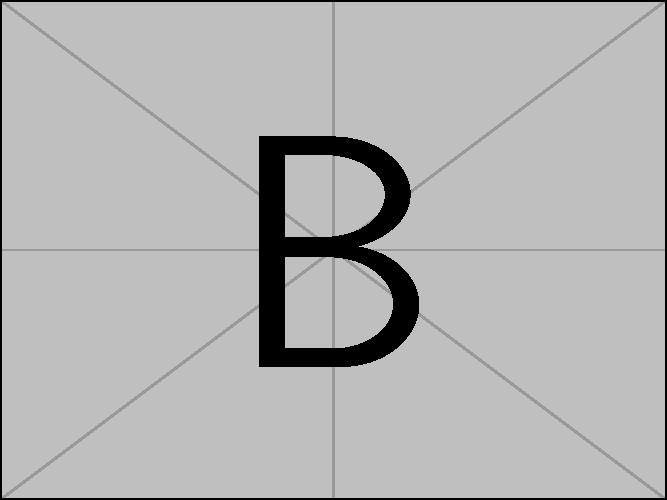
\includegraphics[width=0.35\linewidth]{example-image-b.pdf}}
	\caption{多个分图的示例}
	\label{fig:multi-image}
\end{figure}
\end{python}

效果如下:

\begin{figure}
	\centering
	\subcaptionbox{分图 A\label{fig:subfig-a}}
	{
\includegraphics[width=0.35\linewidth]{example-image-a.pdf}}
	\subcaptionbox{分图 B\label{fig:subfig-b}}
	{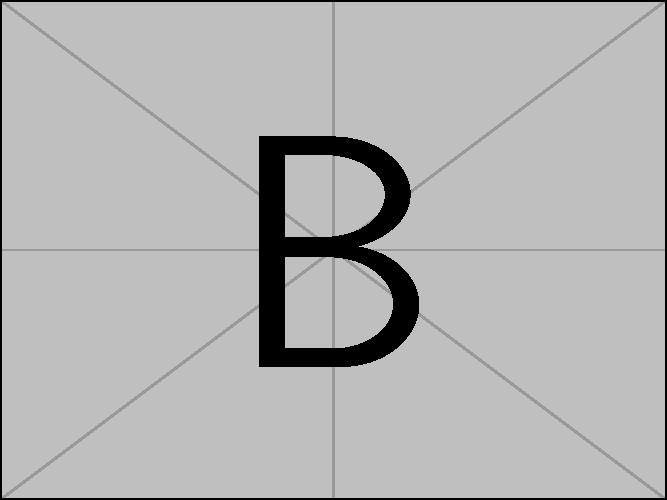
\includegraphics[width=0.35\linewidth]{example-image-b.pdf}}
	\caption{多个分图的示例}
	\label{fig:multi-image}
\end{figure}

\subsection{图片引用}

通过在表格中加入\textbackslash label\{fig\_name\}来定义表格名称,在文本中使用\textbackslash ref\{fig\_name\}来引用。

建议在\textbackslash ref前添加空格~以示美观。

例如:

\begin{python}
此处引用图~\ref{fig:multi-image},及其图~\ref{fig:subfig-b}和图~\ref{fig:subfig-b}。
\end{python}

效果为:

此处引用图~\ref{fig:multi-image},及其图~\ref{fig:subfig-b}和图~\ref{fig:subfig-b}。
% !TeX root = ../shcmthesis-example.tex

\chapter{\LaTeX{} 编译}

LaTex可以使用OverLeaf进行在线编译,或者使用已有的Tex软件进行本地编译。如果是初学者对于安装Tex软件并不熟悉,推荐使用OverLeaf在线编译。

\section{使用OverLeaf在线编译}

OverLeaf是一个使用LaTeX进行多人协同编辑的平台,可以免费注册和使用,不用下载LaTeX软件,是最为著名的LaTeX在线协作系统。主要特色是有LaTeX插件,编辑功能十分完善,有实时预览(即编即看,无需手动编译)的功能。科研工作者可以在各大期刊的网站上下载到其Overleaf模板,进行论文写作。\footnote{节选自\url{https://www.cstcloud.cn/resources/452}}

\subsection{打开文件流程}

下面给出了两种方案,任选一种即可。

\subsubsection{使用OverLeaf模板}

直接打开OverLeaf网站上的模板即可,网址:\url{https://www.overleaf.com/latex/templates/shcmthesis-shang-hai-yin-le-xue-yuan-xue-wei-lun-wen-latex-mo-ban/nmwwrrnkyyxx}

\subsubsection{手动上传至OverLeaf}

1. 打开OverLeaf官网\url{https://www.overleaf.com/},登录/注册用户。

2. 在Project页面内\url{https://www.overleaf.com/project},选择「New Project」(图~\ref{fig:overleaf1}),在下拉选项内选择「Upload Project」(图~\ref{fig:overleaf2})。

\begin{figure}
	\centering
	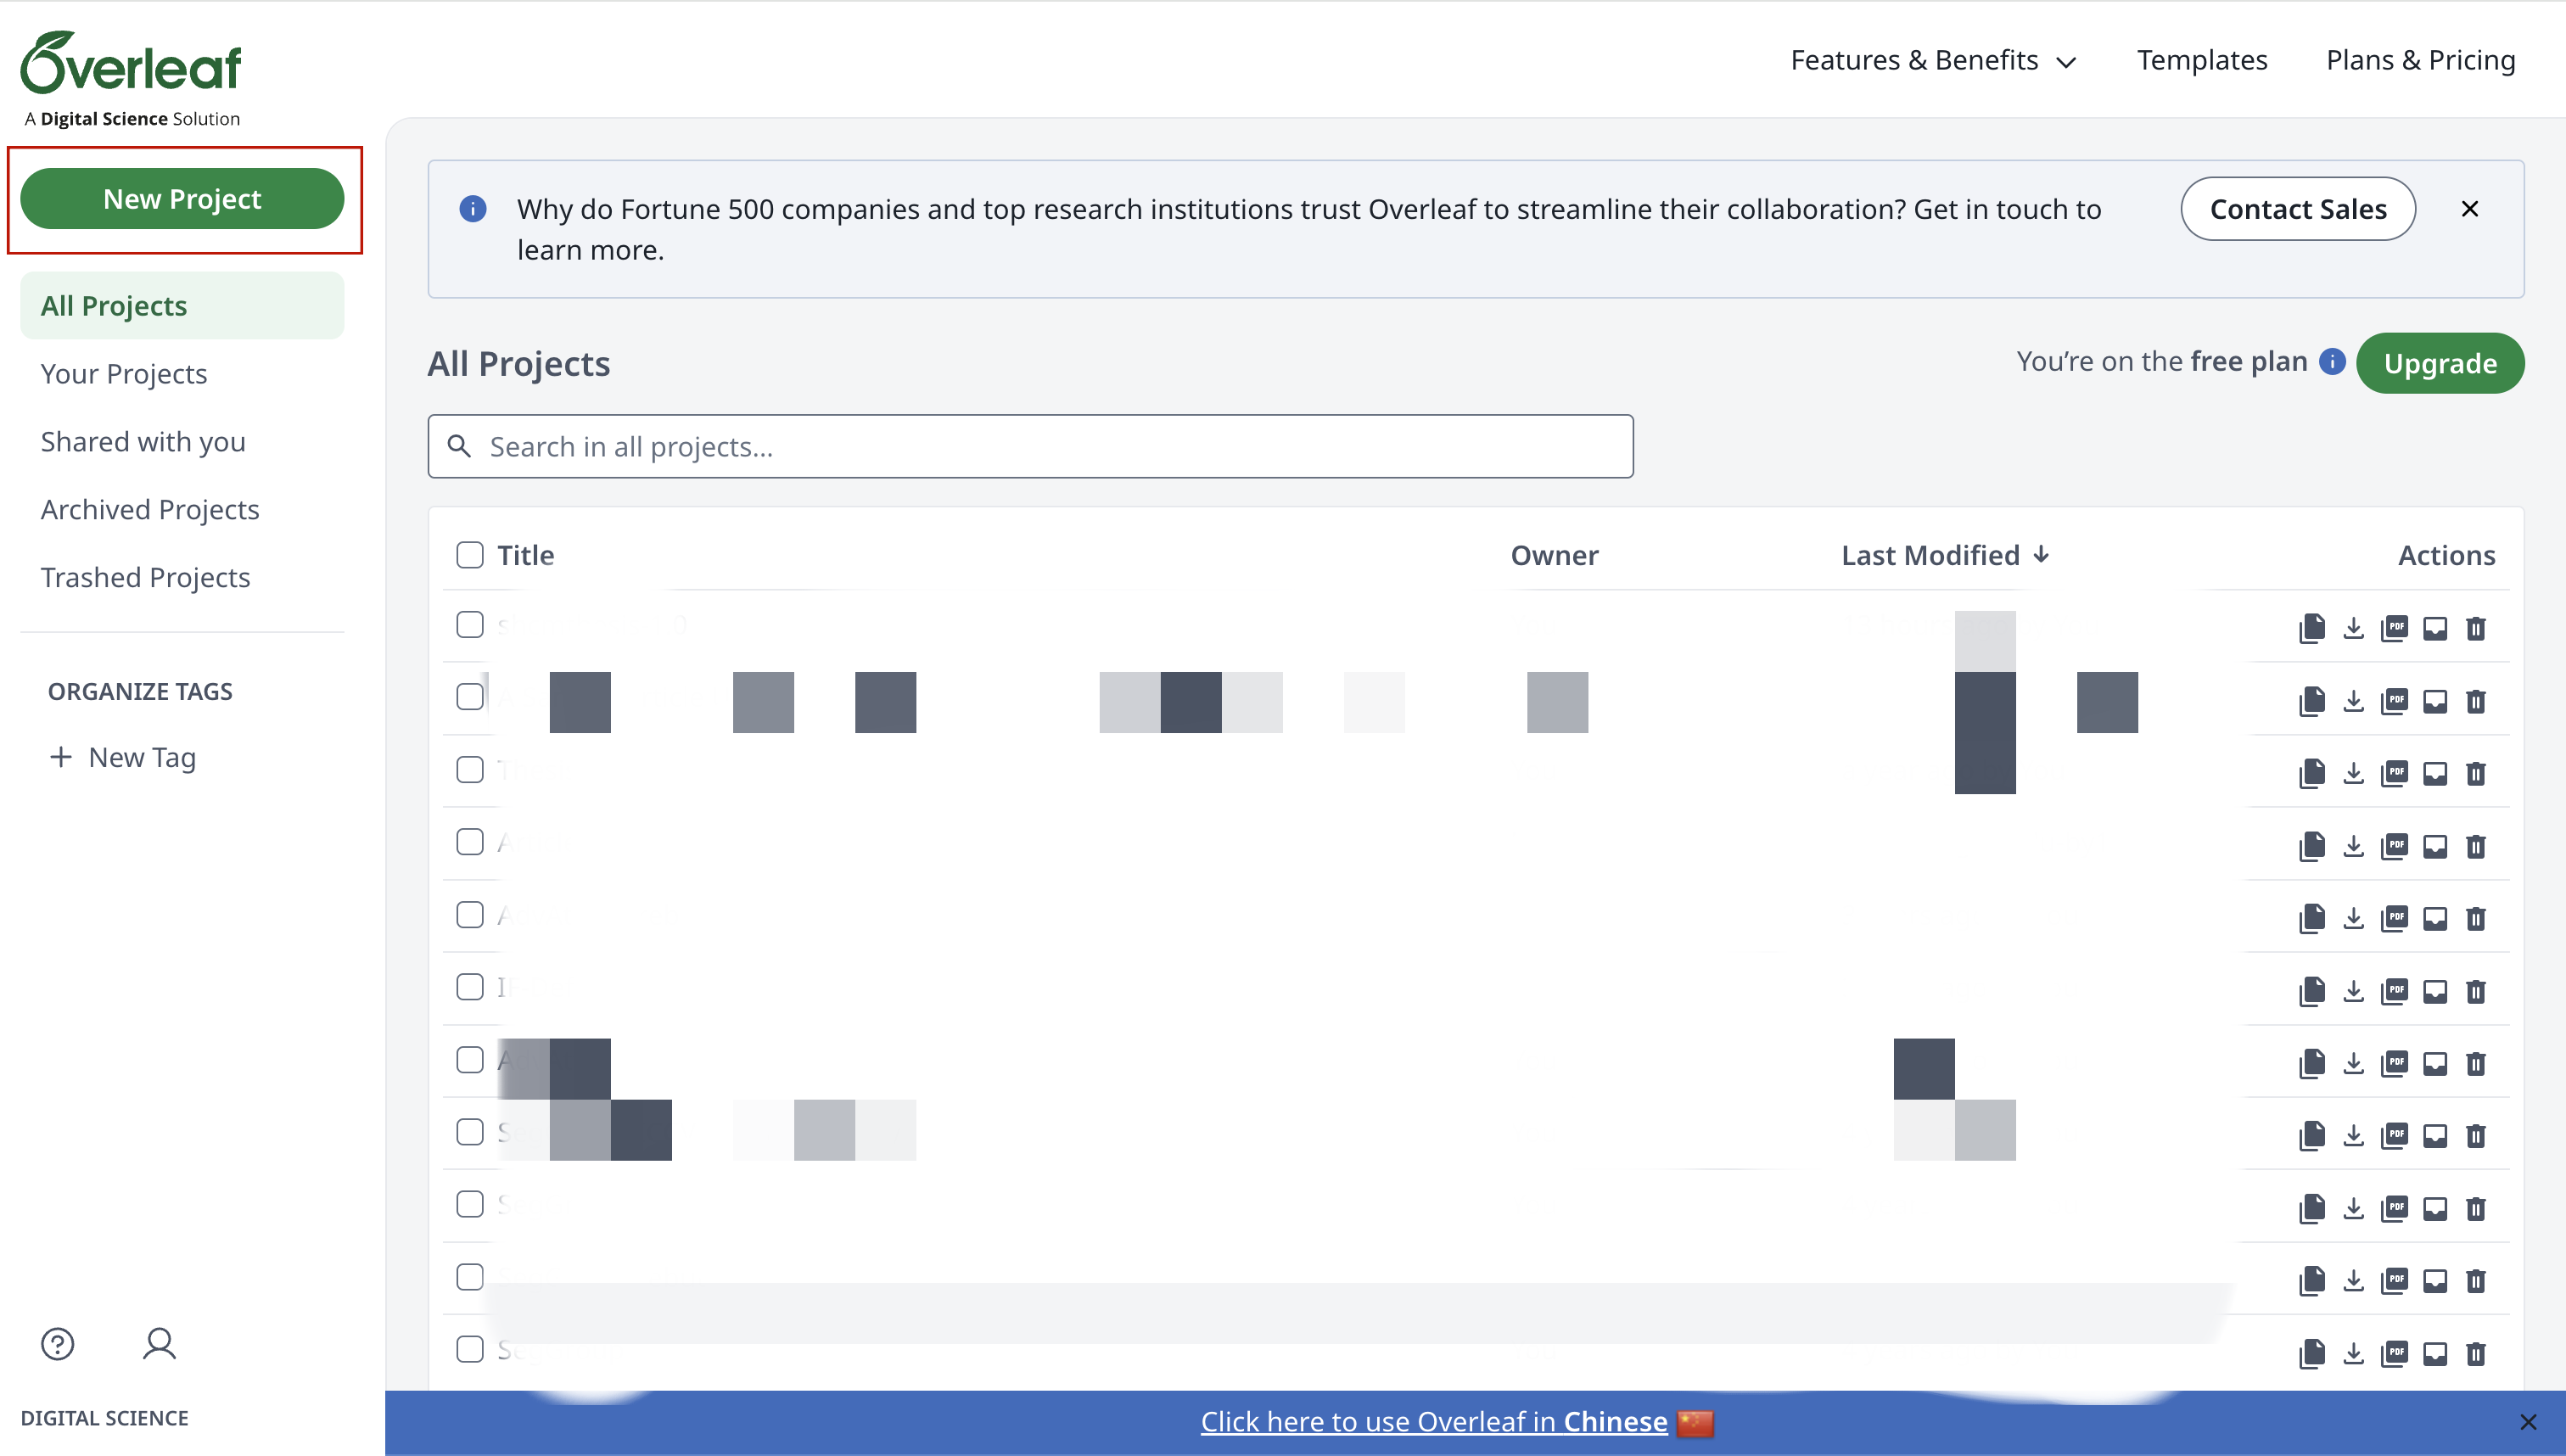
\includegraphics[width=0.5\linewidth]{overleaf/overleaf1}
	\caption{选择「New Project」}
	\label{fig:overleaf1}
\end{figure}

\begin{figure}
	\centering
	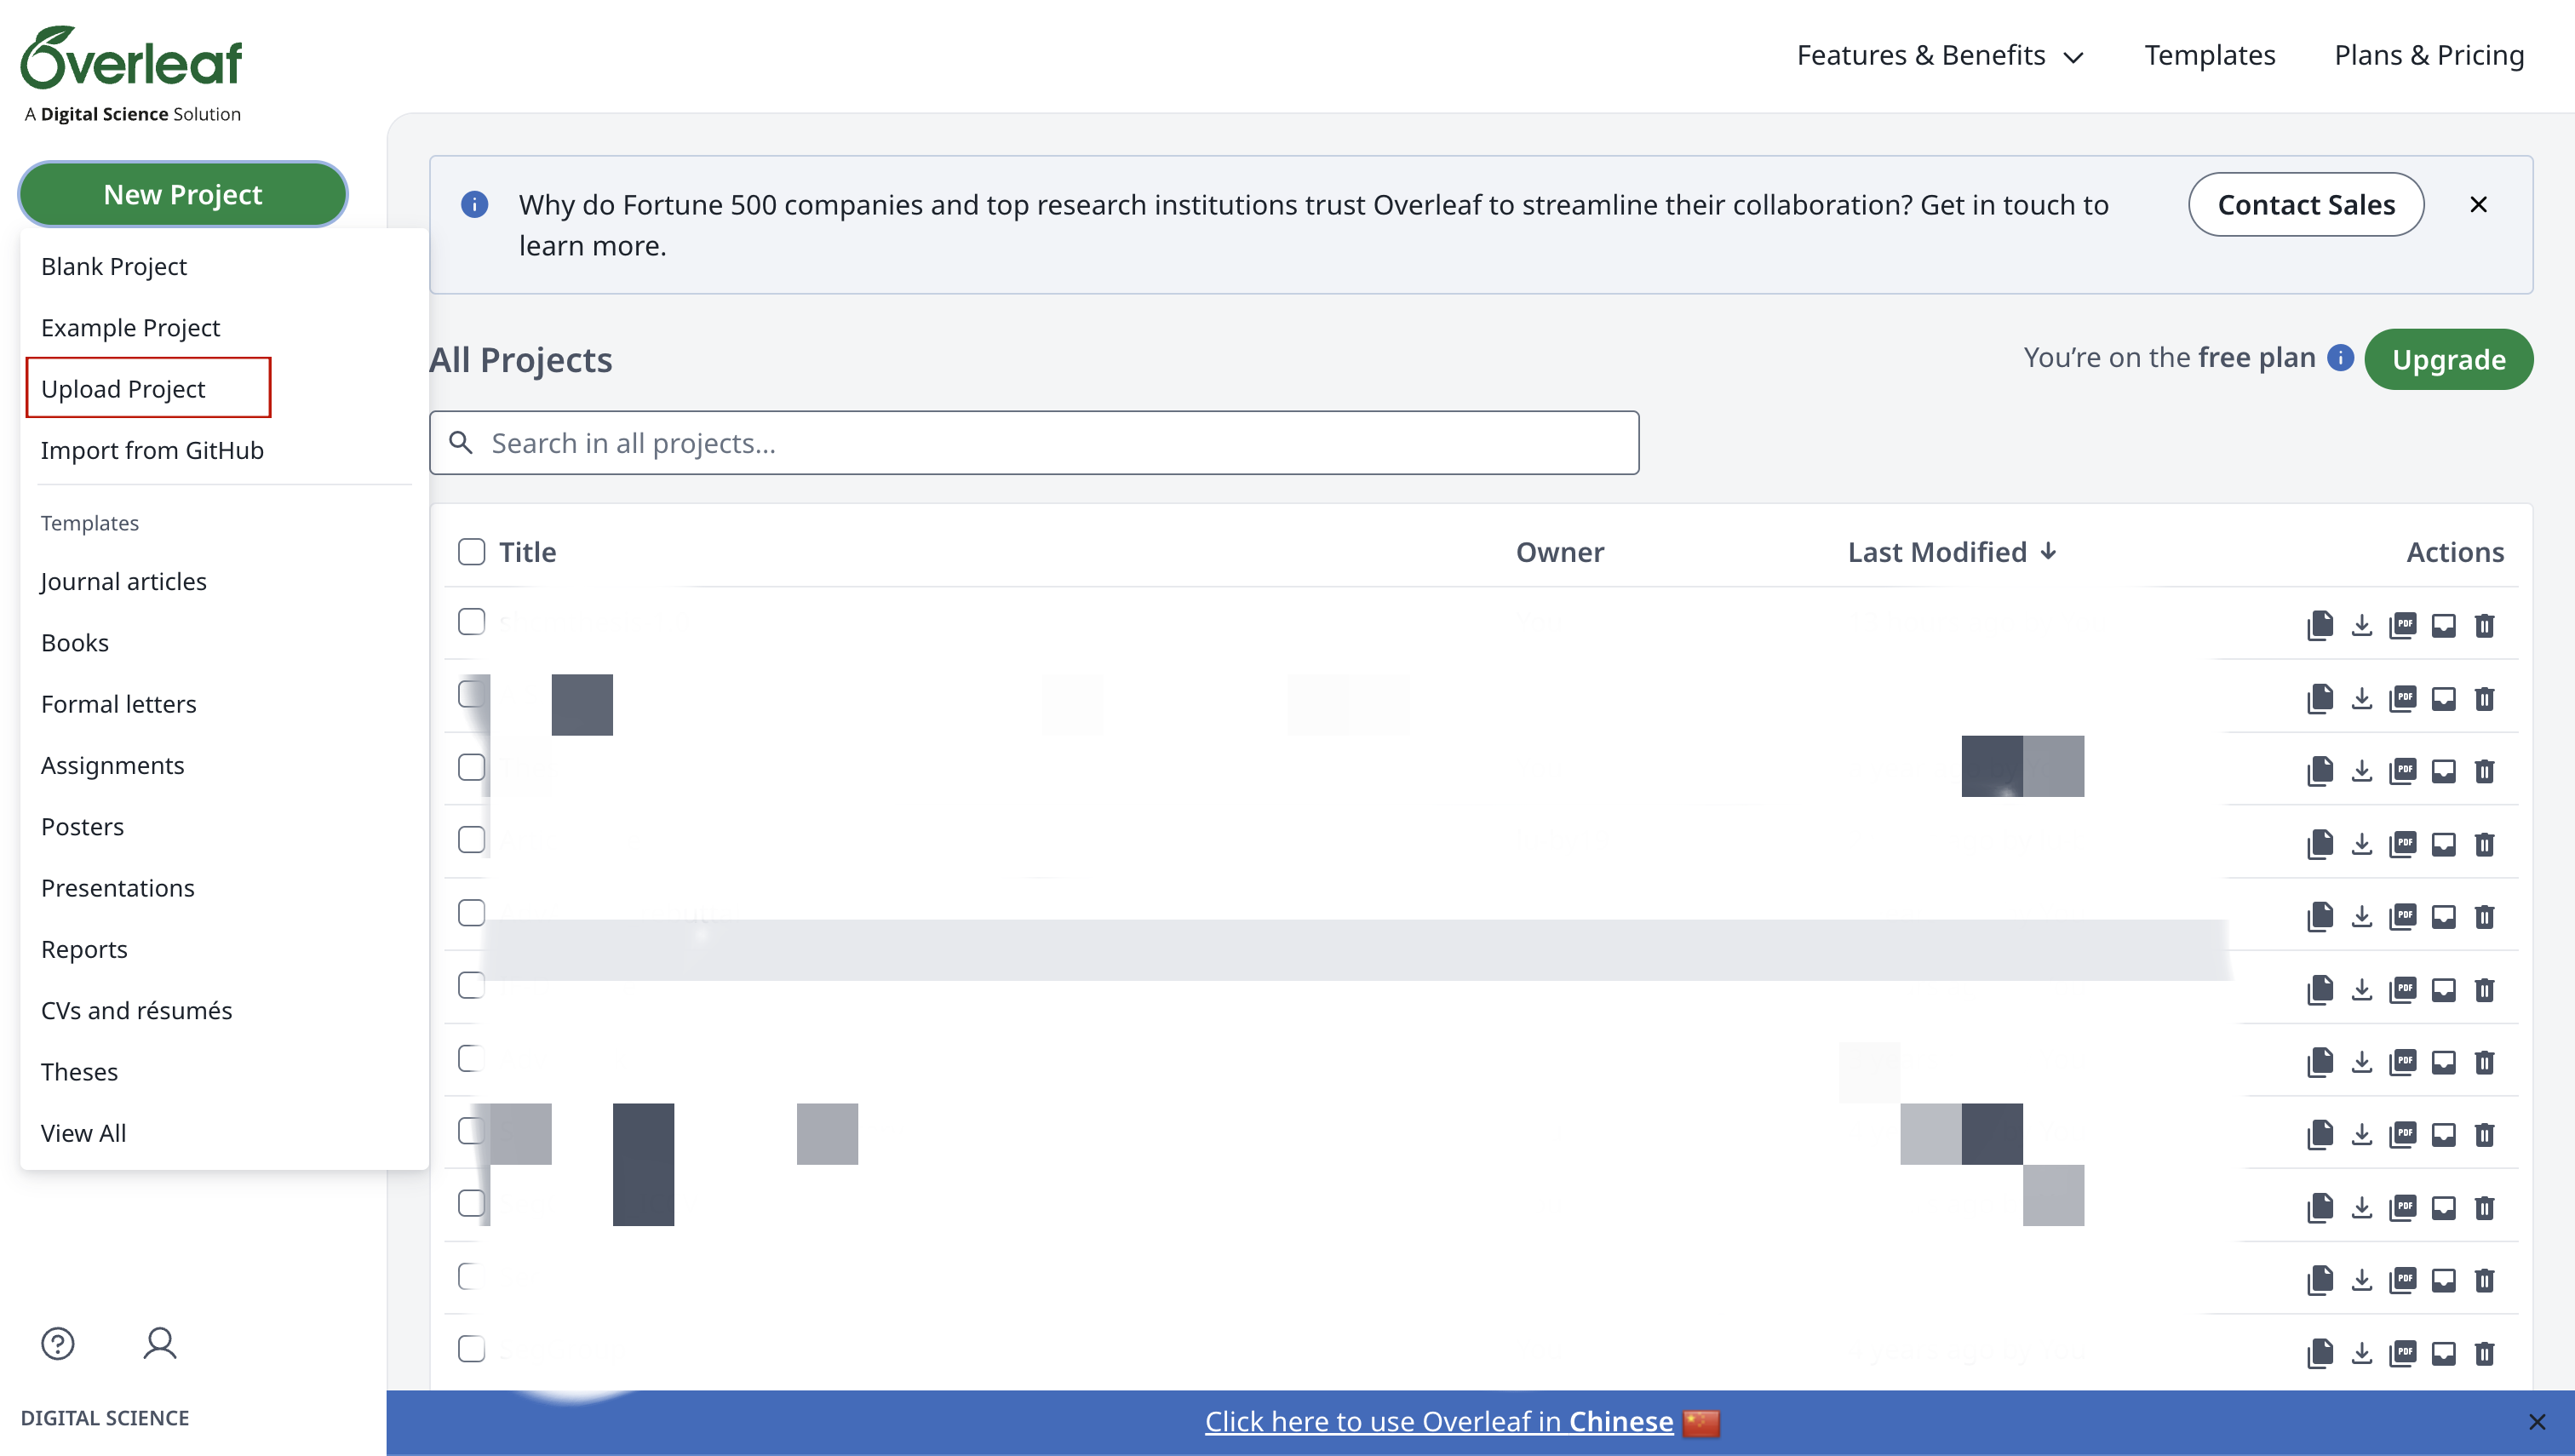
\includegraphics[width=0.5\linewidth]{overleaf/overleaf2}
	\caption{选择「Upload Project」}
	\label{fig:overleaf2}
\end{figure}

3. 将本模板的ZIP包上传至弹出的窗口内(图~\ref{fig:overleaf3})。

\begin{figure}
	\centering
	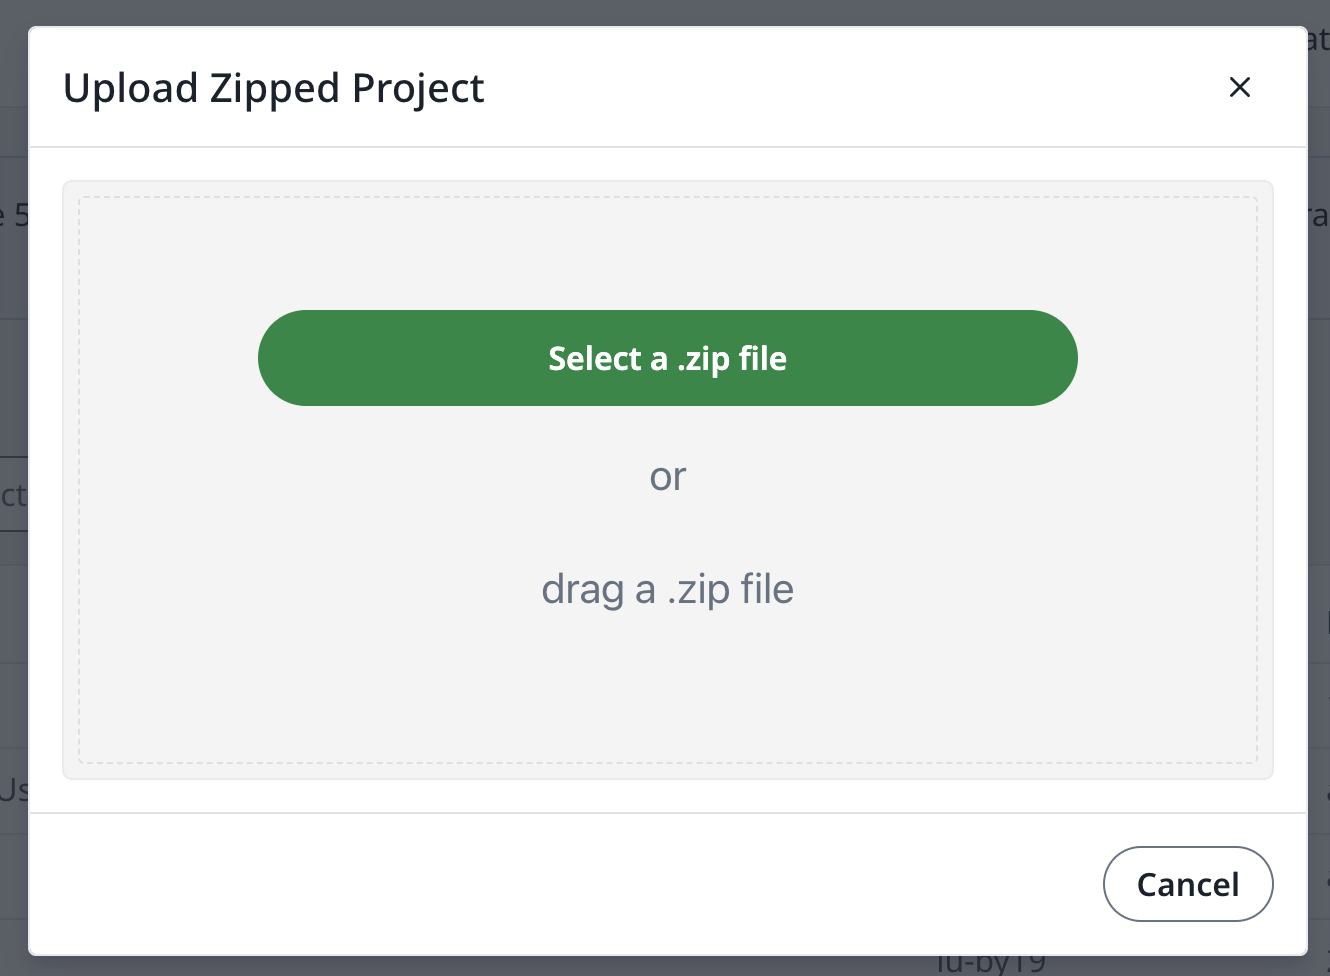
\includegraphics[width=0.5\linewidth]{overleaf/overleaf3}
	\caption{上传ZIP包}
	\label{fig:overleaf3}
\end{figure}

4. 打开项目后,打开「Menu」(图~\ref{fig:overleaf4_1}),在「Settings」的「Compiler」,将「PdfLaTex」(图~\ref{fig:overleaf5_1})改成「XeLaTex」(图~\ref{fig:overleaf6})。

\begin{figure}
	\centering
	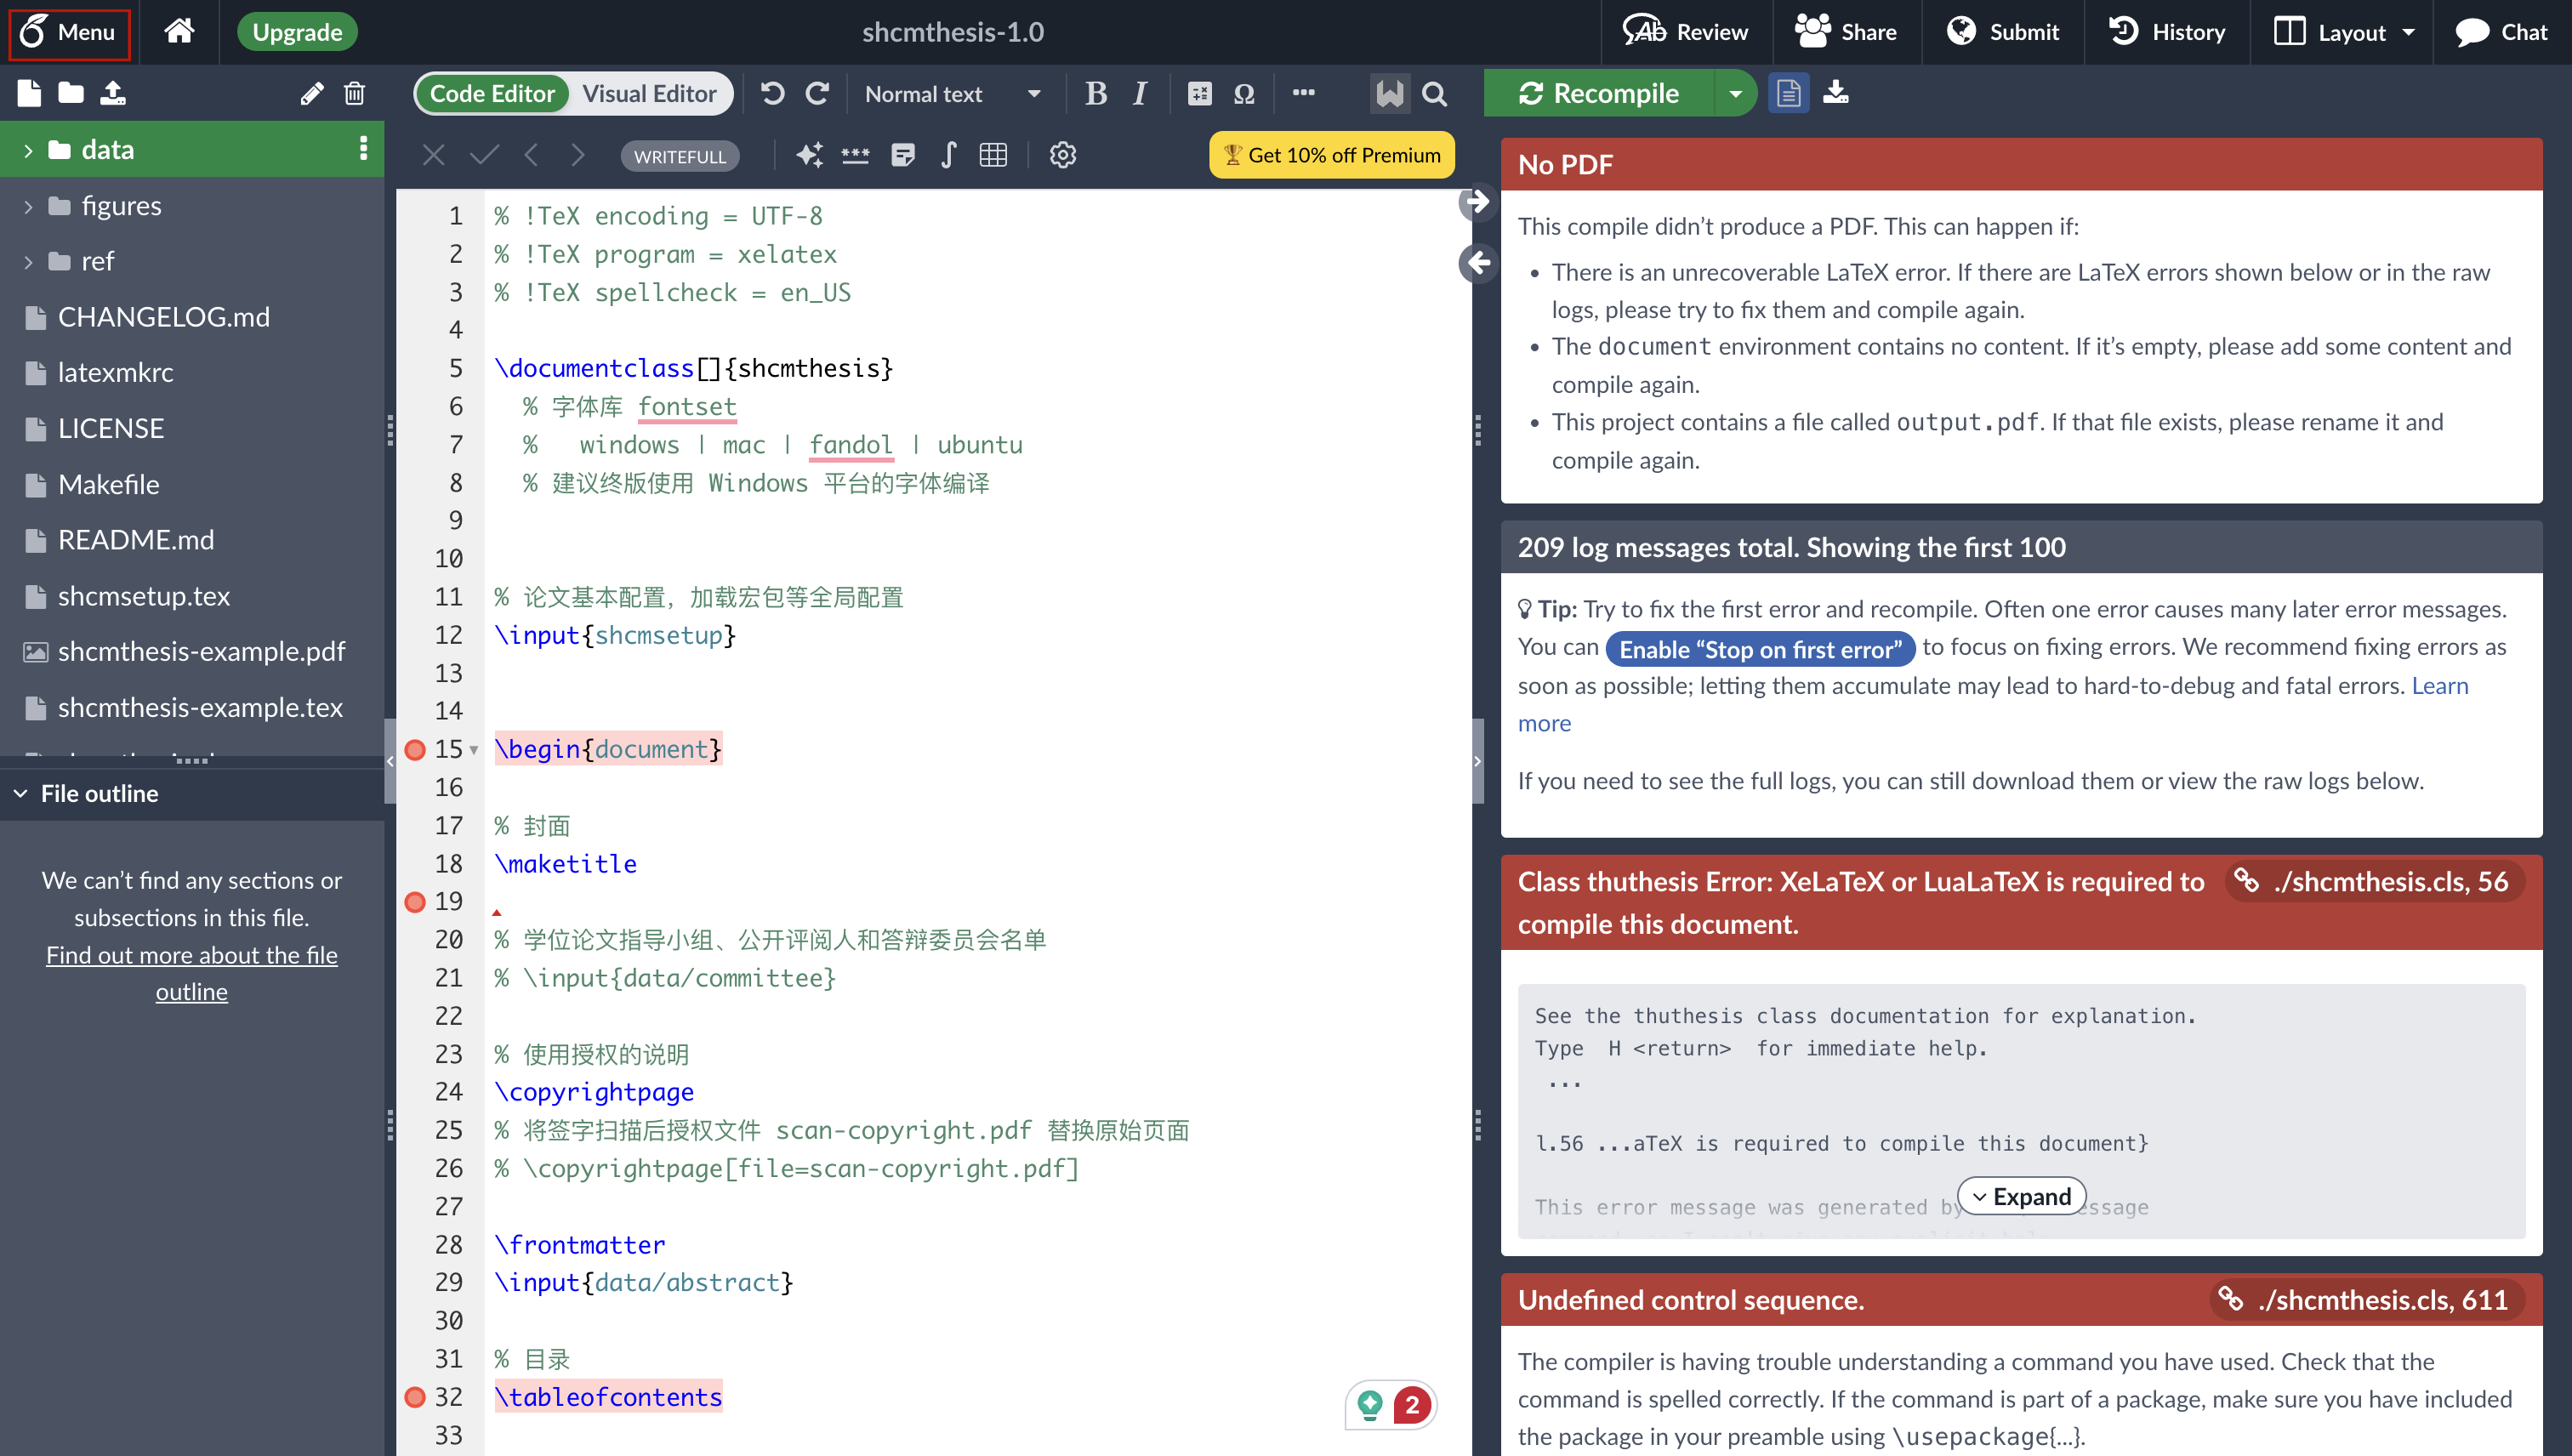
\includegraphics[width=0.5\linewidth]{overleaf/overleaf4_1}
	\caption{打开「Menu」}
	\label{fig:overleaf4_1}
\end{figure}

\begin{figure}
	\centering
	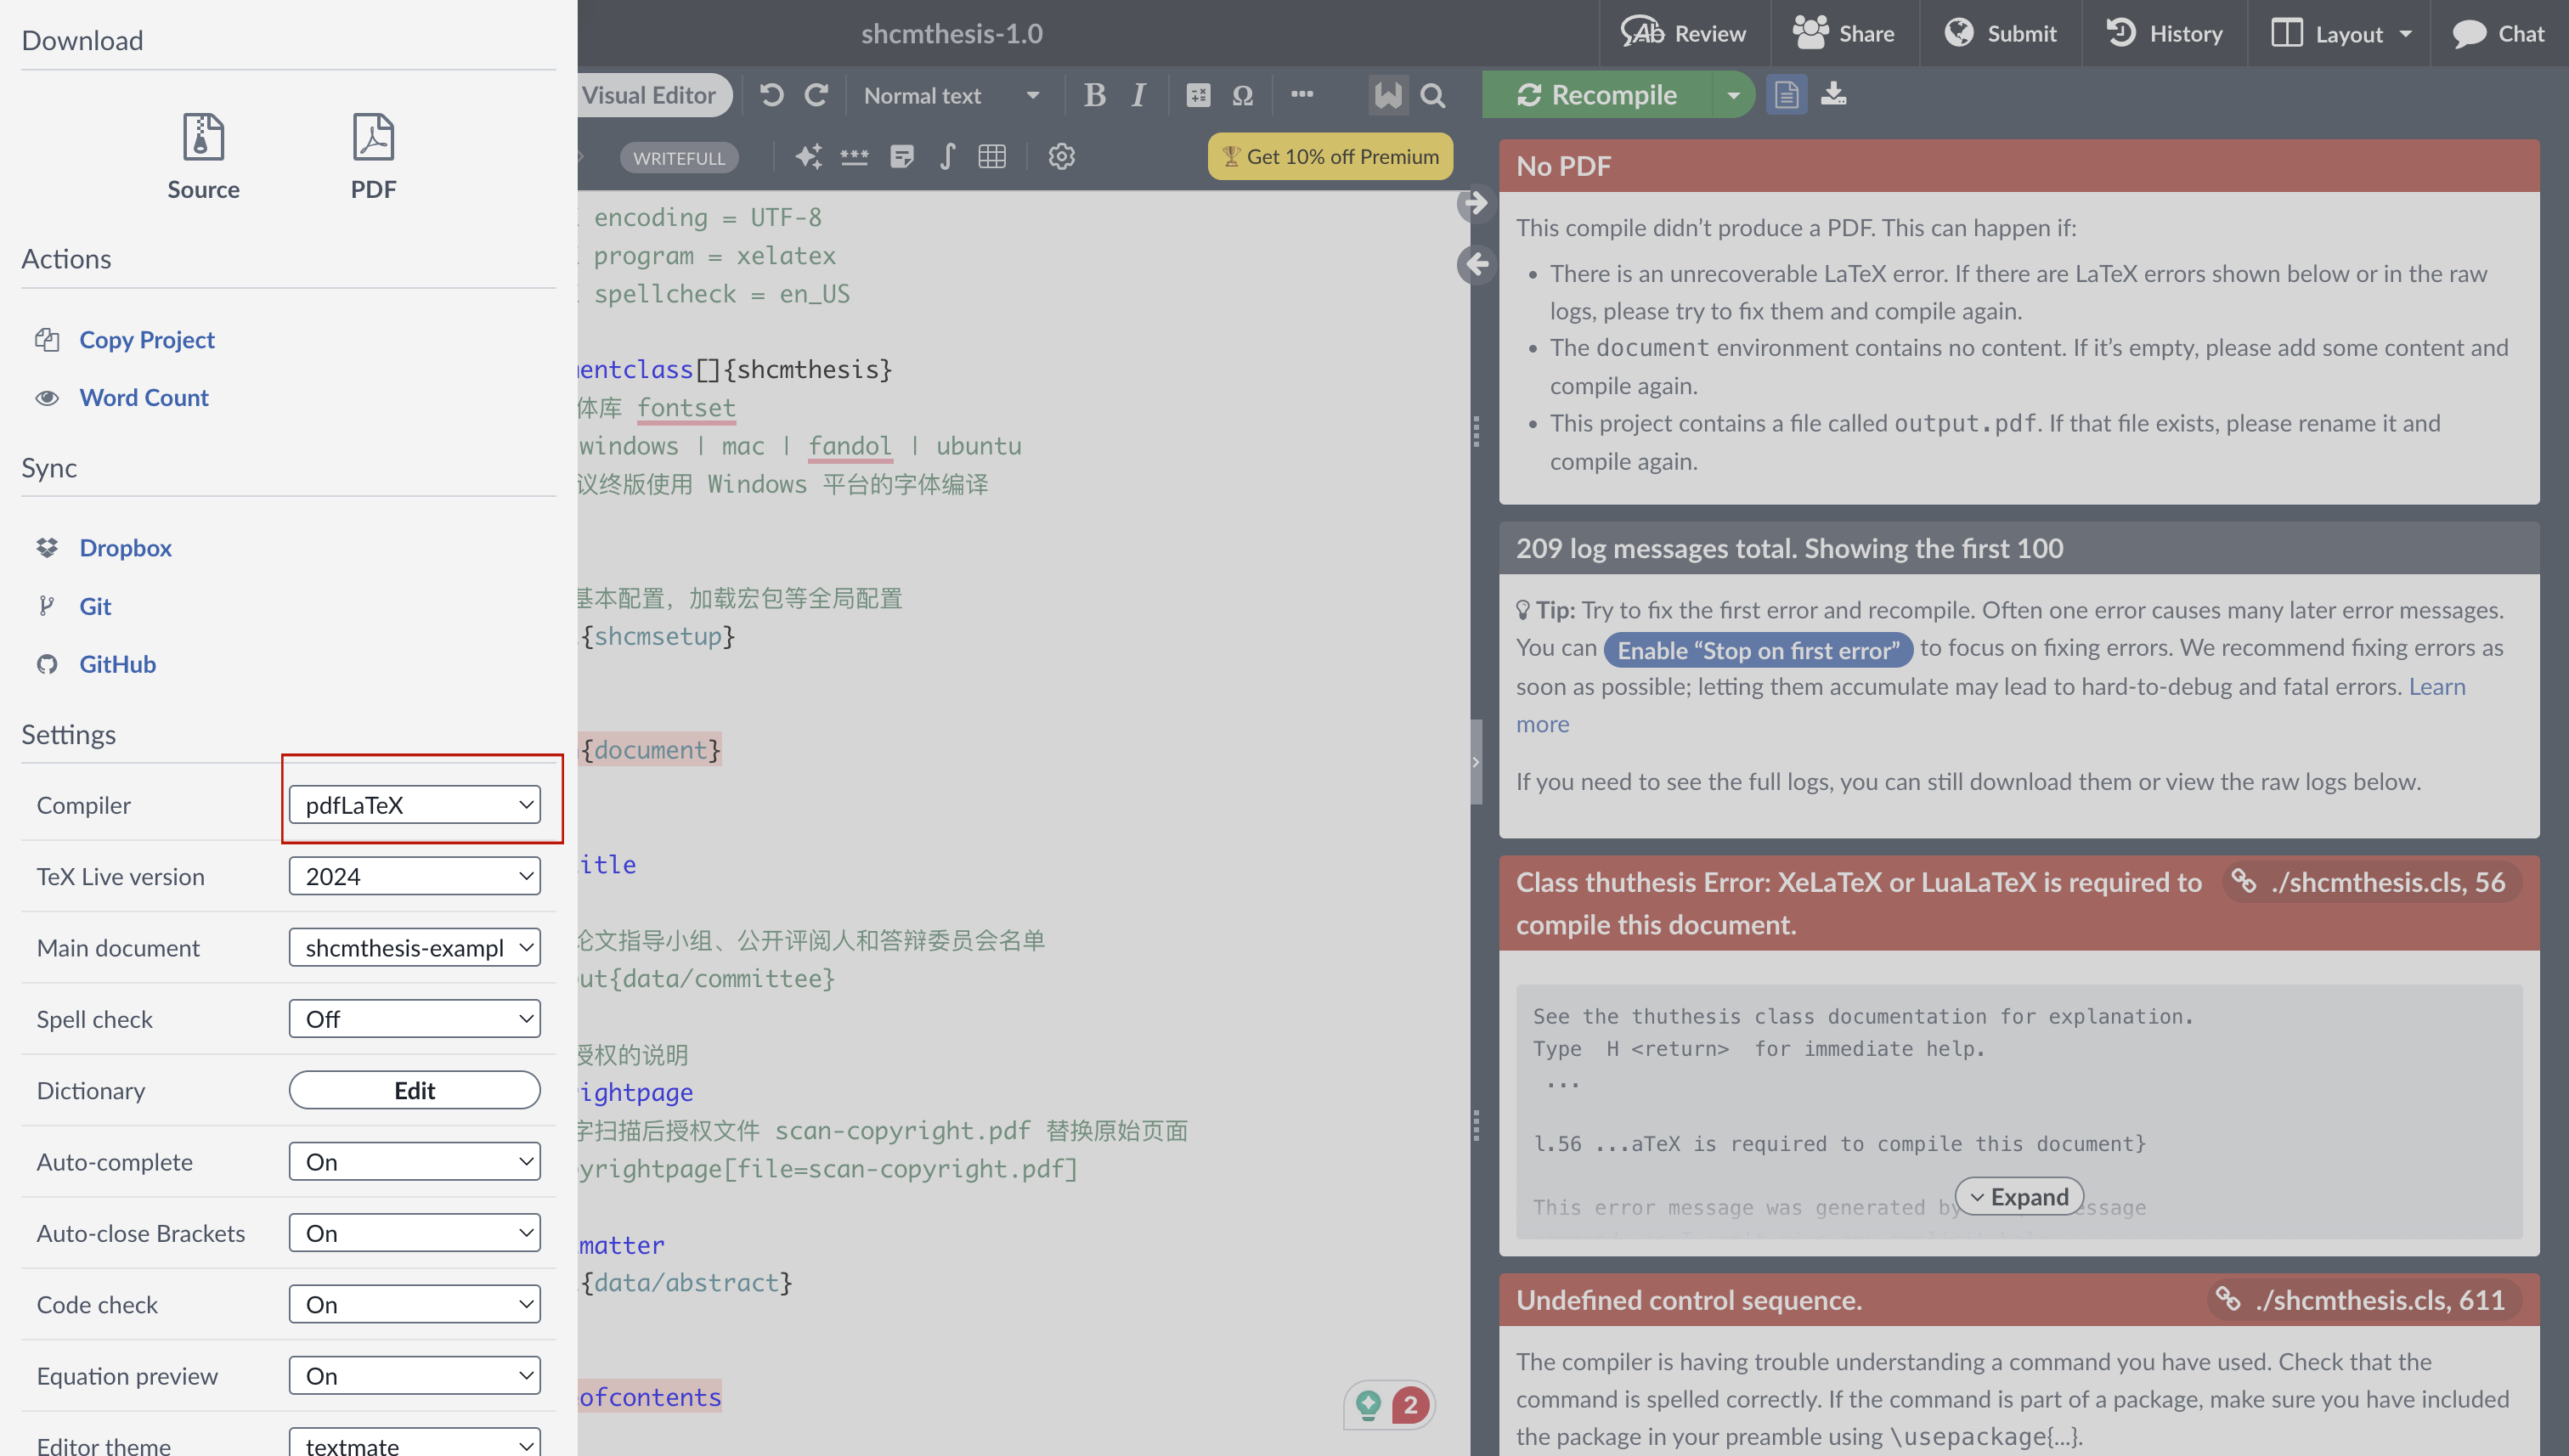
\includegraphics[width=0.5\linewidth]{overleaf/overleaf5_1}
	\caption{原先设置为「PdfLaTex」}
	\label{fig:overleaf5_1}
\end{figure}

\begin{figure}
	\centering
	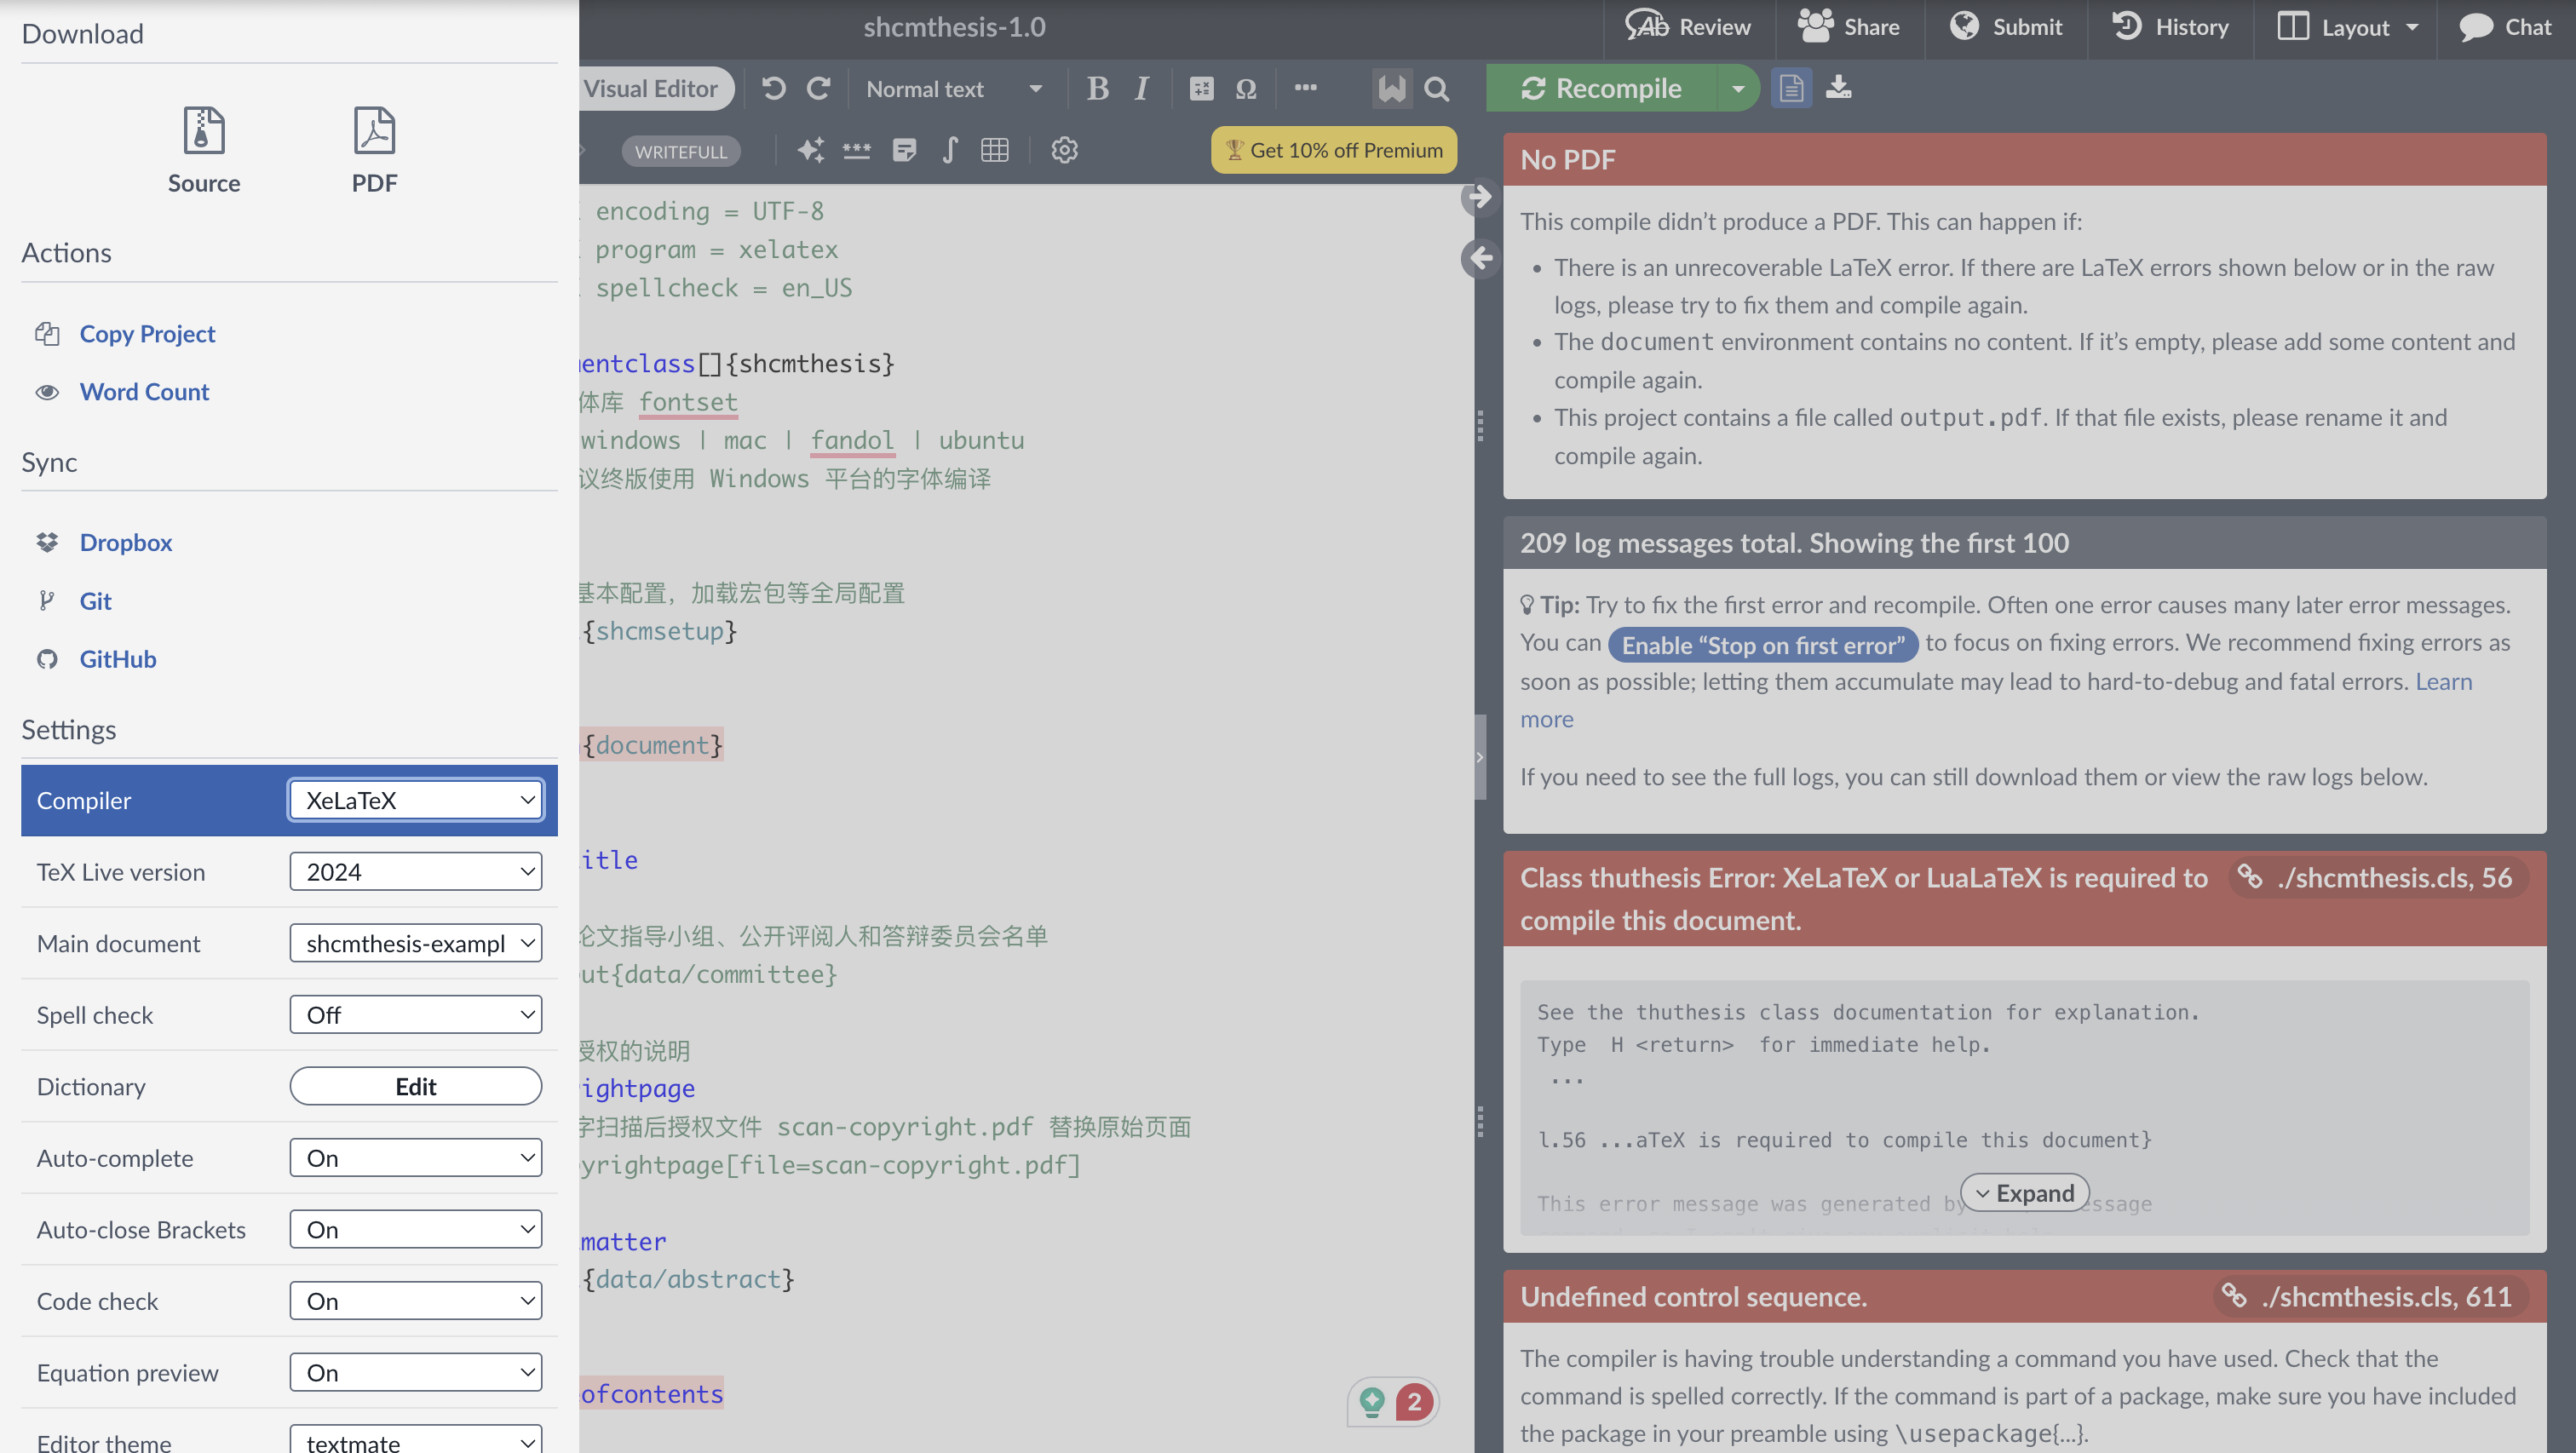
\includegraphics[width=0.5\linewidth]{overleaf/overleaf6}
	\caption{更改为「XeLaTex」}
	\label{fig:overleaf6}
\end{figure}

5. 在页面右侧视图的左上点击「Recompile」进行编译(图~\ref{fig:overleaf4_2}),即可生成PDF文件。

\begin{figure}
	\centering
	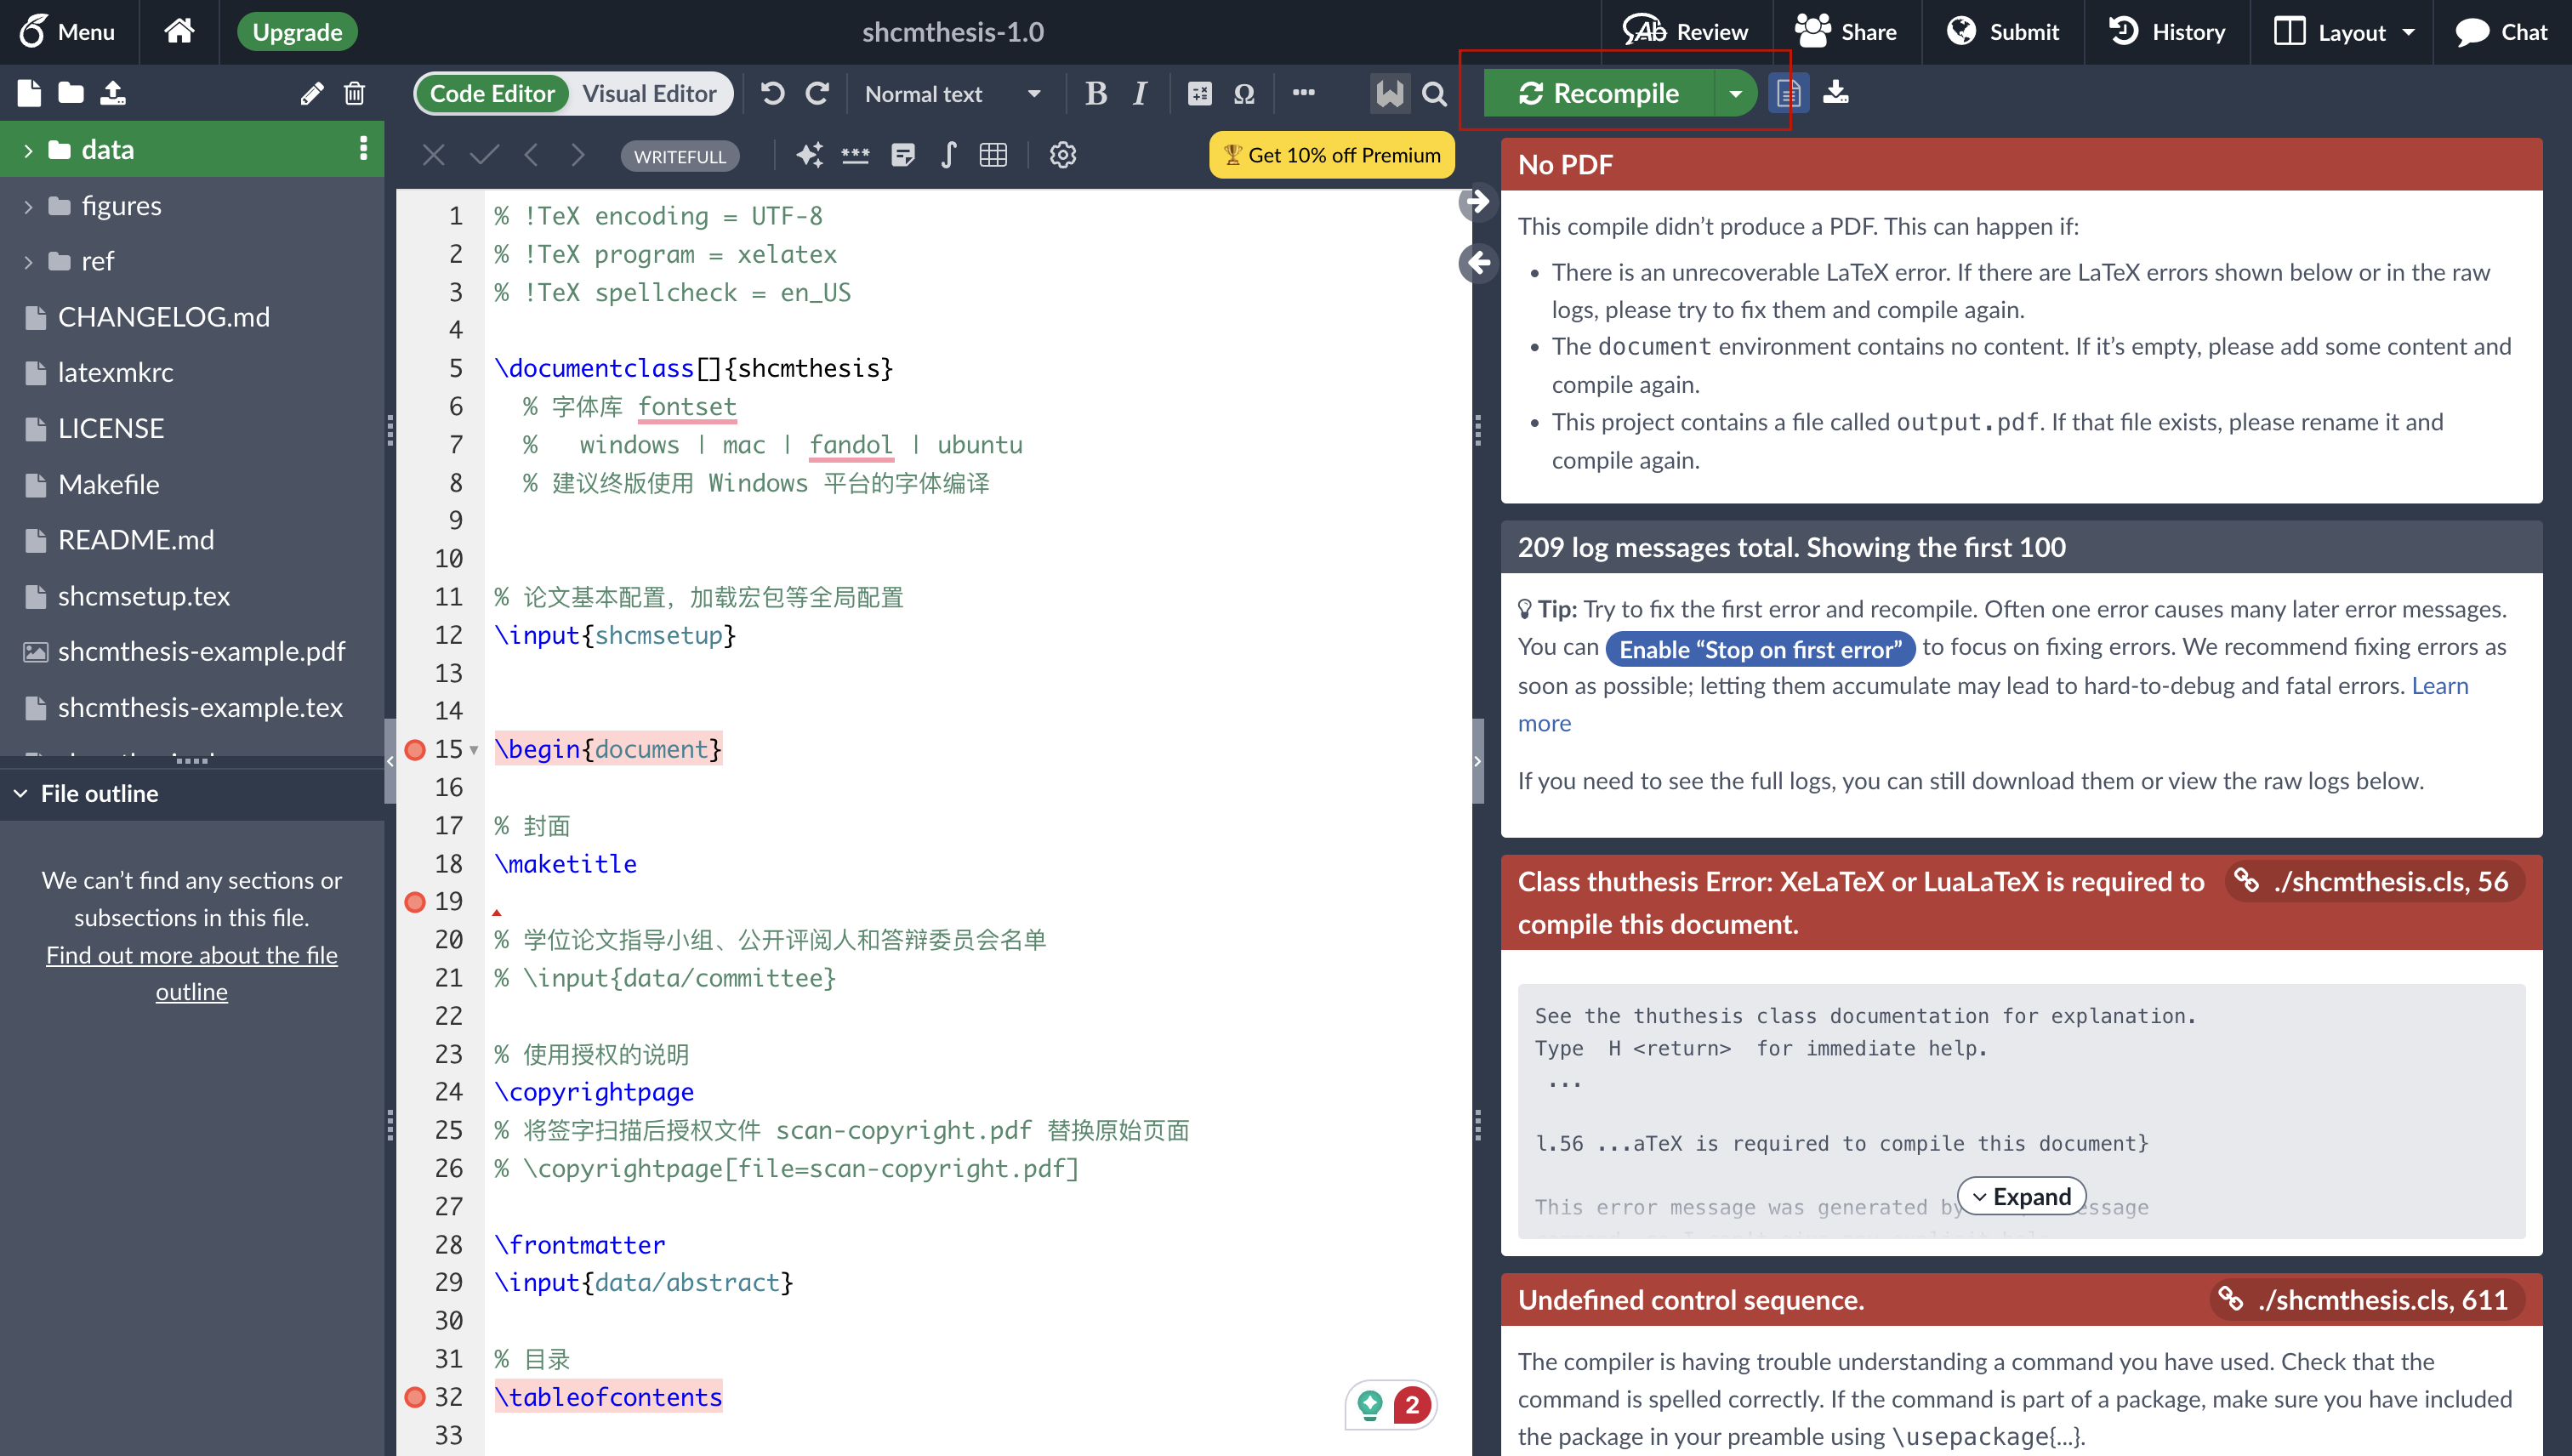
\includegraphics[width=0.5\linewidth]{overleaf/overleaf4_2}
	\caption{点击「Recompile」进行编译}
	\label{fig:overleaf4_2}
\end{figure}

\subsection{使用介绍}

1. 更改文本内容之后,可以点击「Recompile」重新进行编译生成PDF文件(图~\ref{fig:overleaf4_2})。

2. 可以通过左右箭头对应正在编辑的文字与PDF中的位置(图~\ref{fig:overleaf7})。

\begin{figure}
	\centering
	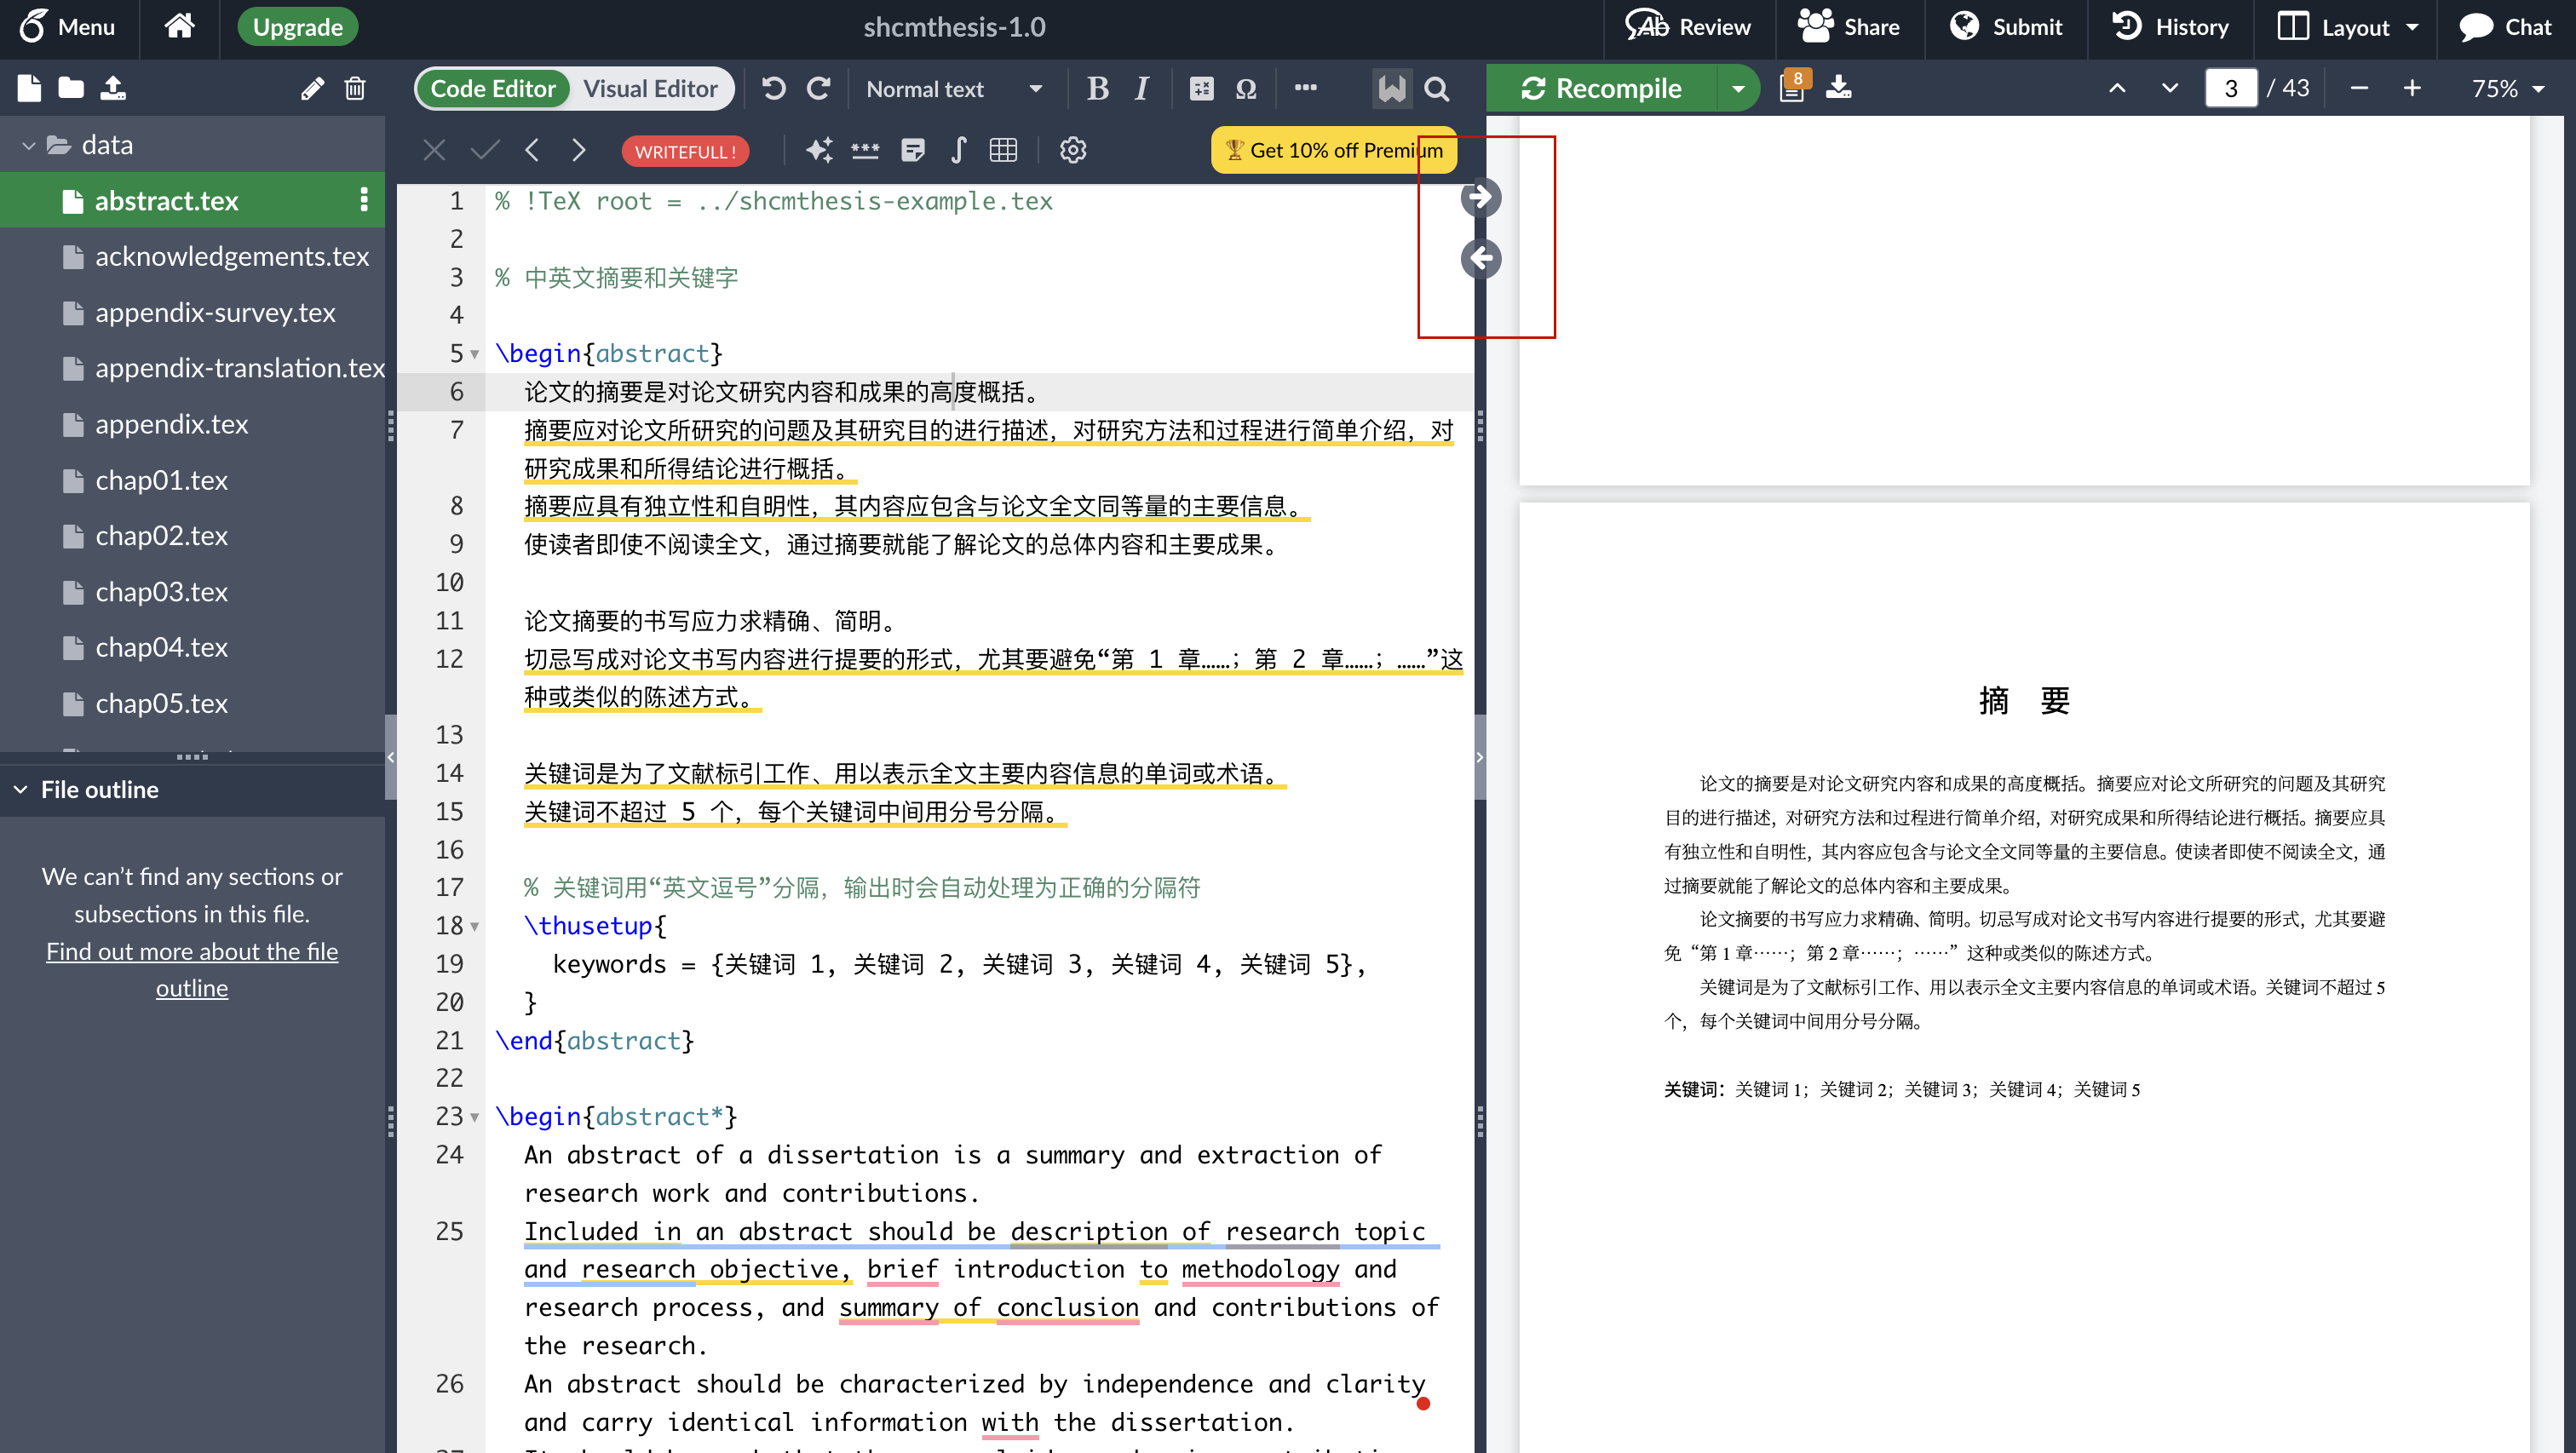
\includegraphics[width=0.5\linewidth]{overleaf/overleaf7}
	\caption{通过左右箭头对应正在编辑的文字与PDF中的位置}
	\label{fig:overleaf7}
\end{figure}

3. 由于OverLeaf为在线编译器,网站可能会瘫痪(很少见),因此建议随时做好备份。在「Menu」内可以随时下载全部文件(Source)或者生成的PDF文件(PDF)(图~\ref{fig:overleaf5_2})。

\begin{figure}
	\centering
	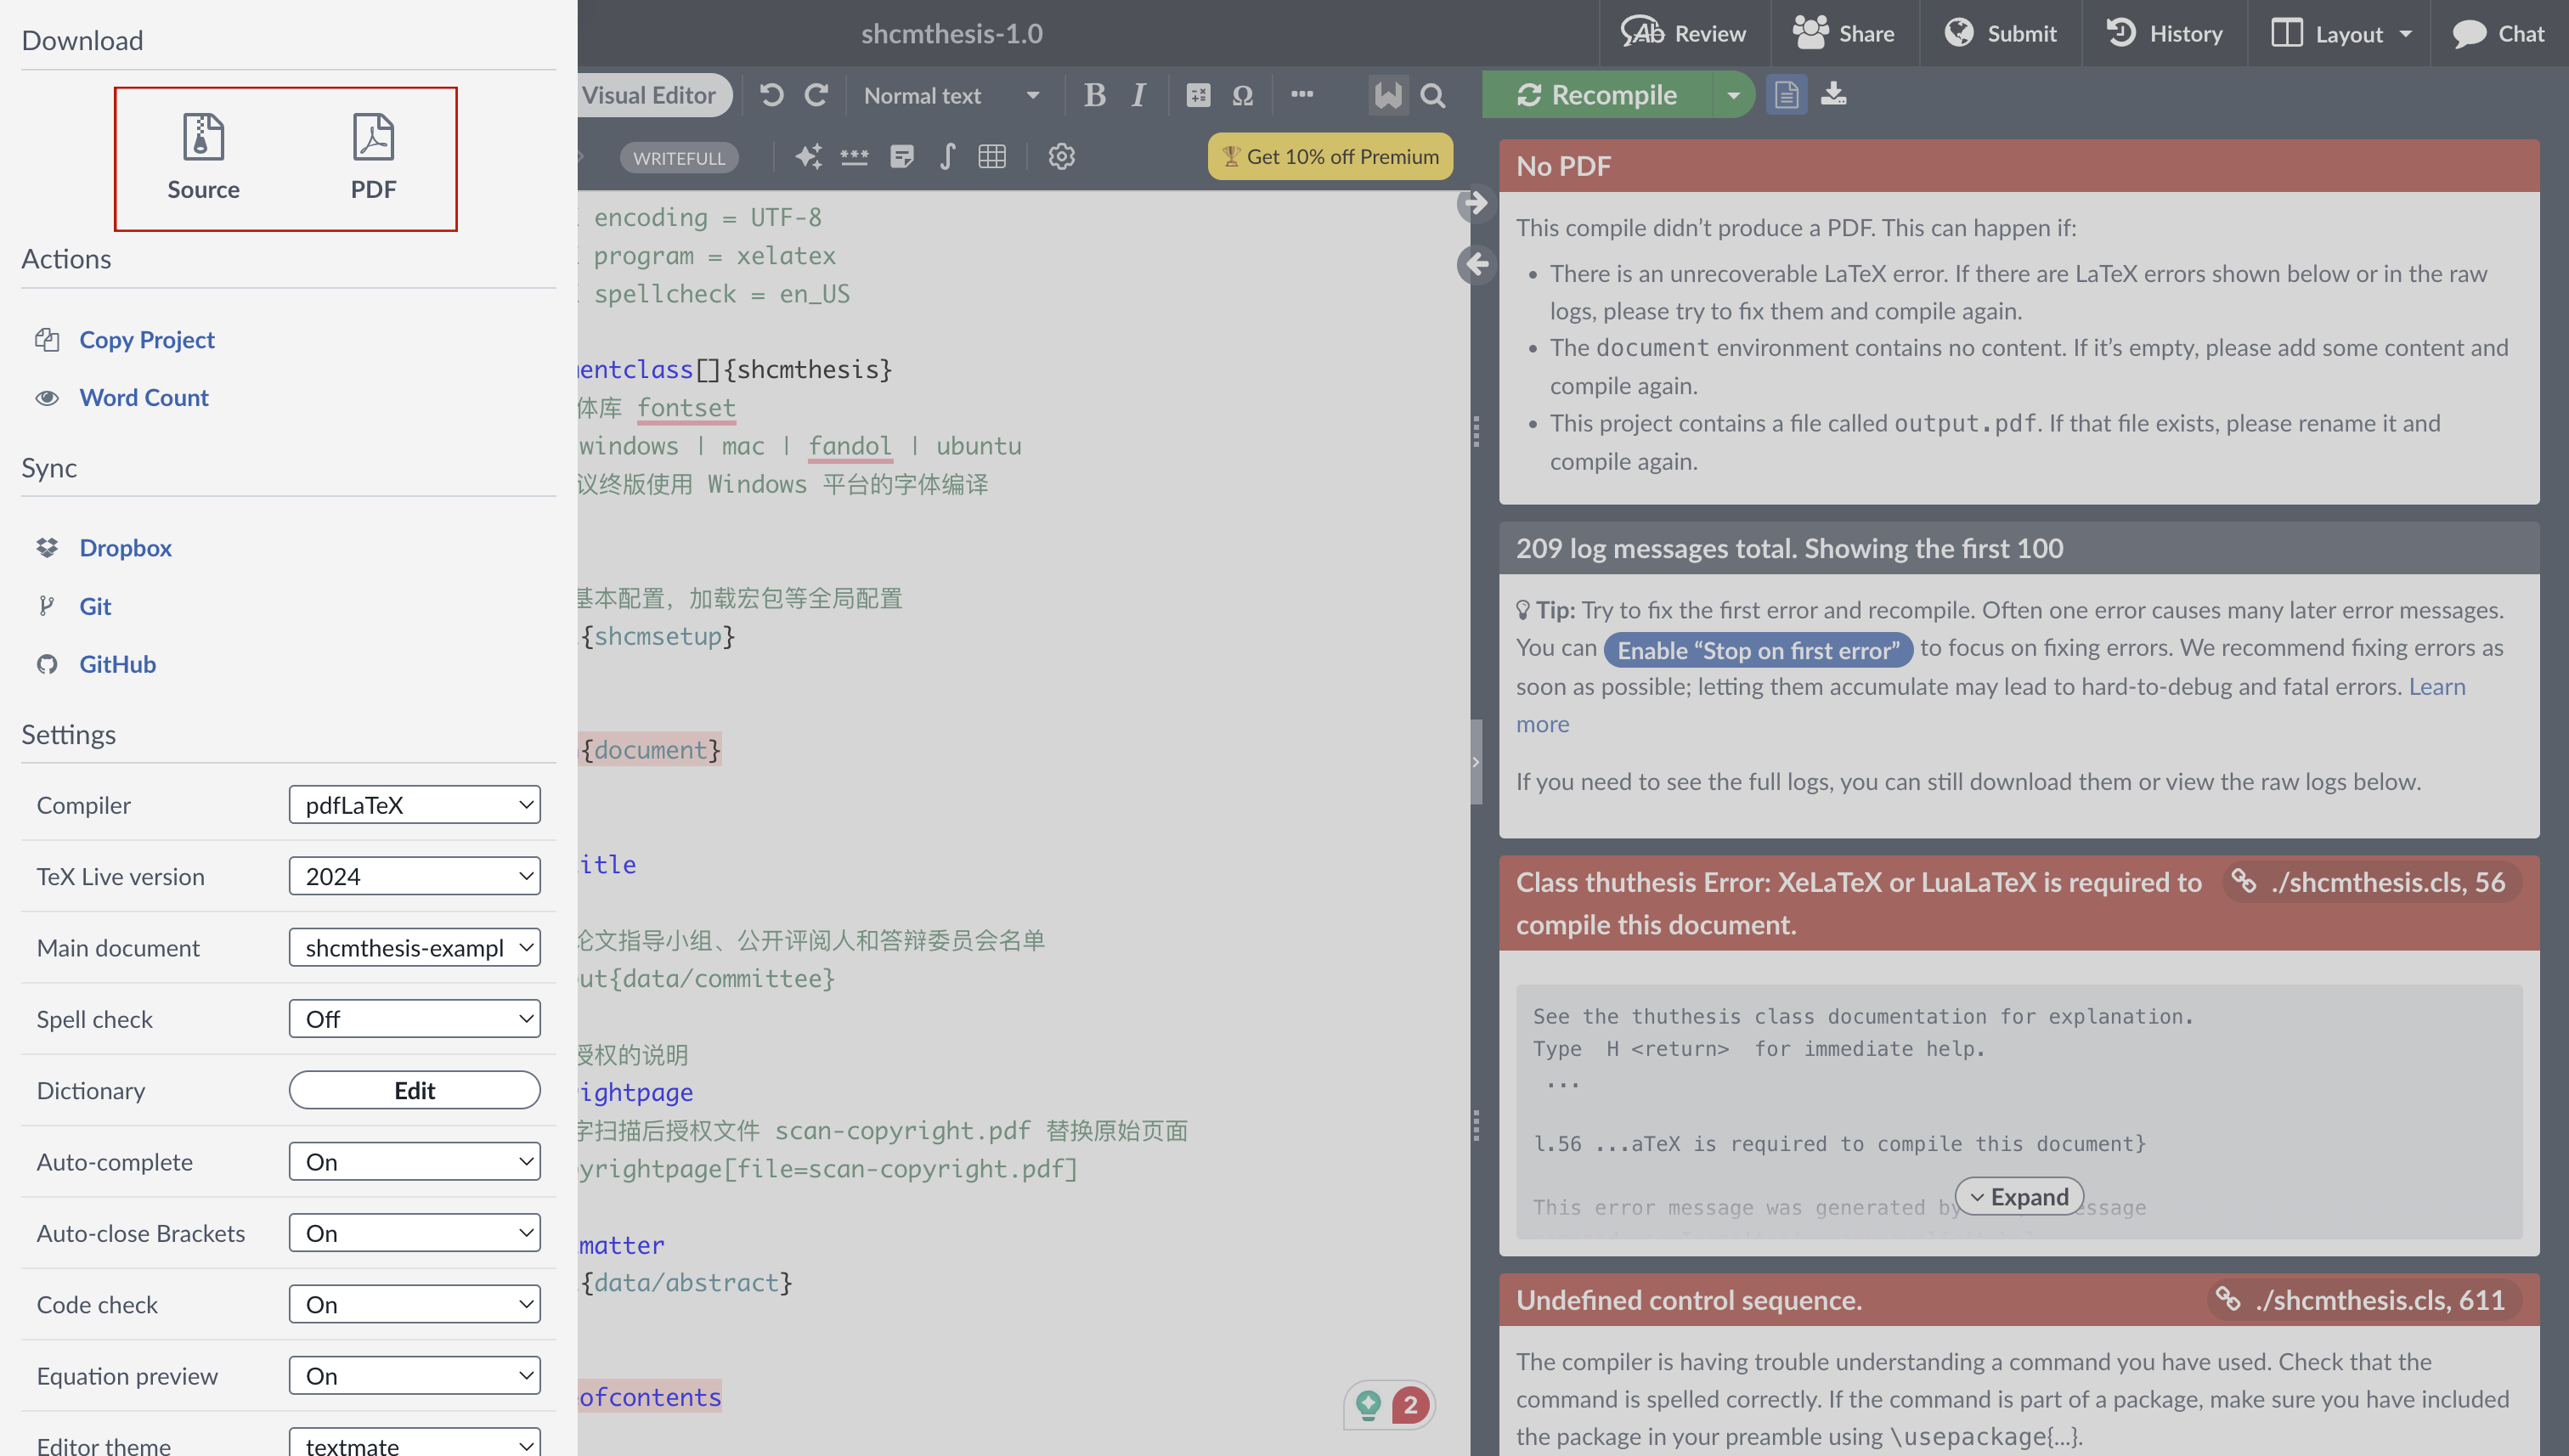
\includegraphics[width=0.5\linewidth]{overleaf/overleaf5_2}
	\caption{下载全部文件(Source)或者生成的PDF文件(PDF)}
	\label{fig:overleaf5_2}
\end{figure}

\section{使用Tex本地编译}

\textbf{声明:以下文字节选复制自\url{https://oi-wiki.org/tools/latex/},并根据本文情况稍作修改}

对于 Windows 用户,你需要下载 TeX Live 或 MikTeX。国内用户可以使用 清华大学 TUNA 镜像站(\url{https://mirrors.tuna.tsinghua.edu.cn/}),请点击页面右侧的「获取下载链接」按钮,并选择「应用软件」标签下的「TeX 排版系统」即可下载 TeX Live 或 MikTeX 的安装包,其中 TeX Live 的安装包是一个 ISO 文件,需要挂载后以管理员权限执行 install-tl-advanced.bat。

对于 macOS 用户,清华大学 TUNA 镜像站同样提供 MacTeX 和 macOS 版 MikTeX 的下载。

对于 Linux 用户,如果使用 TeX Live,则同样下载 ISO 文件,执行 install-tl 脚本;如果使用 MikTeX,则按照 官方文档(\url{https://miktex.org/download\#unx}) 进行安装。

安装完成后,同样需要选择编译器为XeLaTex。

\section{文档结构说明}

下面介绍本模板的各个文件的功能和使用方式。

\subsection{全局信息设置}

本模板的标题作者信息设置位于shcmsetup.tex,请根据自己的信息进行修改。

需要设置的变量如下:

\subsubsection{输出格式:}

选择打印版(print)或用于提交的电子版(electronic),前者会插入空白页以便直接双面打印。

待赋值变量:output

\subsubsection{封面格式:}

选择用于预审(preliminary)或用于最终提交的终版(final)

待赋值变量:cover

\subsubsection{学位类型:}

选择本科(bachelor)、硕士(master)或者博士(doctor),会影响封面不同,其他部分不影响。

待赋值变量:degree

\subsubsection{论文标题:}

-1和-2分别对应标题的第一行和第二行,加*的为英文标题

待赋值变量:title-1、title-1、title-1*、title-2*

\subsubsection{论文编号:}

待赋值变量:thesis-id

\subsubsection{学科专业:}

待赋值变量:discipline

\subsubsection{作者姓名:}

待赋值变量:author

\subsubsection{作者学号:}

待赋值变量:student-id

\subsubsection{指导教师:}

中文姓名和职称之间以英文逗号“,”分开,例如`{李红,教授}`。

待赋值变量:supervisor

\subsubsection{完成日期:}

待赋值变量:date

\subsection{文字内容填写}

本模板的所有文字内容位于data/目录下,各文件所代表正文部分如下:

摘要(中英文):data/abstract.tex

符号和缩略语说明:data/denotation.tex

正文:

\indent \indent 章节1:data/chap01.tex

\indent \indent 章节2:data/chap02.tex

\indent \indent 章节3:data/chap03.tex

\indent \indent 章节4:data/chap04.tex

\indent \indent 章节5:data/chap05.tex

参考文献:data/ref.tex

附录:data/appendix.tex

致谢:data/acknowledgements.tex

%如果编译不出最新修改的内容,请尝试删除shcmthesis-example.bbl、shcmthesis-example.lof、shcmthesis-example.lot、shcmthesis-example.out、shcmthesis-example.toc、shcmthesis-example.aux、shcmthesis-example.synctex.gz、shcmthesis-example.pdf这些文件,然后重新编译。

\subsection{图片文件}

本模板的所有图片内容位于figures/目录下,可根据需要自行添加新的图片。

% !TeX root = ../shcmthesis-example.tex

\part{上海音乐学院研究生学位论文写作规范}
\chapter{总纲}

\textbf{声明:以下部分所有内容均复制自《上海音乐学院研究生学位论文写作规范》\footnote{https://yjsb.shcmusic.edu.cn/\_t3/2023/0315/c2687a46645/page.htm}。}\\

学位论文是研究生科研工作成果的集中体现,是研究生培养学位工作的重要环节,是申请博士、硕士学位的主要依据,也是社会重要的文献资料。为进一步促进我院研究生学位论文的规范化,保证研究生学位论文的质量和学位论文文本的科学性和规范性,根据中华人民共和国国家标准GB/T 7713.1-2006《学位论文编写规则》、GB/T 7714-2015《文后参考文献著录规则》及《中国高等学校社会科学学报编排规范》等文件精神,结合我院实际,制订此写作规范。

% !TeX root = ../shcmthesis-example.tex

\chapter{研究生学位论文基本要求}

\section{学位论文内容方面撰写要求}

学位论文应在导师指导下独立完成,且不能以在读期间该生导师及其作品作为学位论文研究对象,不得抄袭他人的文字或剽窃他人的研究成果。论文的选题和所研究的内容应在学术上有一定的理论意义和实践意义。学位申请人对论文所涉及的研究课题,应具有较为坚实的基础理论和专业知识。对前人在相同或相似课题上已经取得的研究成果应有比较全面的了解和认识。申请人应掌握论文研究课题所必须的研究方法和技能。

博士论文要求对所研究的课题具有系统性、学术性和前瞻性,在凸显本专业学科特性的同时,鼓励在研究方法上有所创新;学术型硕士论文要求对所研究的课题有新的见解,专业学位硕士论文要有一定的实践总结性。

论文的论据要充分翔实,所用材料须正确可靠。词句要精练,条理清晰;陈述和论证要有逻辑性;谱例图表运用要准确、恰当。论文中所有引用他人的词句,必须作相应的注释。引用文字与作者本人文字之间应保持合理的平衡,避免过度引用。若以综述或转述的方式引用他人的观点或研究成果,也须以注释的方式引证原文或提供原著作名称及相应的页码。对引文的注释内容至少应包括作者姓名、著作名称、出版社或期刊名称、出版或发表的日期和页码。凡大量引用他人词句而不加引号和注释的,均可视为抄袭行为。参考书目应列出作者姓名、著作名称、出版社名称、出版时间。中国古代文献要注明版本来源和出处。申请人在读期间所编著的教学参考书、校注、读书报告和对自己作品的分析研究等,均不得作为学位论文提交。

\section{学位论文摘要撰写要求}

研究生学位论文摘要是学位论文内容不加注释和评论的短篇陈述,应具有相对的独立性和完整性。研究生学位论文摘要应突出本文的新见解和创造性成果。

研究生学位论文摘要应包括中、英文两部分,英文摘要应是中文摘要的全文翻译。学位论文摘要无须单独装订,须装订在版权页(独创性声明)后。
% !TeX root = ../shcmthesis-example.tex

\chapter{研究生学位论文形式和规范要求}

\section{论文基本结构(按先后顺序排列)}

研究生学位论文应由封面、版权页(独创性声明和论文使用授权说明)、中英文摘要、关键词、目录、绪论、正文、结论、参考文献、附录(非必须)、致谢(或后记,非必须)、封底等部分依次组成。

\subsection{封页、纸张及页面设计}

论文封面和封底使用研究生部统一规定样式,可由本院研究生部网页下载版式,按提示的部位、字体、字号等格式要求进行填写(注:博士论文的英文为Dissertation,硕士论文的英文为Thesis)。其中,论文题目要简明扼要,引人注目,以不超过20字为宜,必要时可加用副标题。题名应该避免使用不常见的缩略词、首字母缩写字、字符、代号或公式等。

艺术硕士专业学位论文题目,正标题一般不超过20个字(可另加副标题)。论文题目中不要出现“浅谈”“初探”“浅论”等字样,可用“论”“研究”“探析”等表述。建议直接表述研究的对象和问题。

页面纸张尺寸选择A4型,即21厘米×29.7厘米。页面边距选择“普通”,即上下2.54厘米,左右3.18厘米。

\subsection{版权页(学位论文学术规范声明和学位论文使用授权书)}

为了维护学校、导师及研究生的合法权益,我院所有提出答辩申请的研究生都必须在其学位论文主体内容前附《上海音乐学院博(硕)学位论文学术规范声明》及《上海音乐学院博(硕)学位论文使用授权书》两项内容,以上两项内容放在一个版面页上。在答辩前提交学位论文和答辩后提交留存论文时,以上两项内容上应由研究生本人和导师在相应位置上签名。

\subsection{摘要}

摘要是论文内容的高度概括与简短陈述,应说明本文的目的、研究方法、成果和结论,要突出论文的创造性成果或新见解。语言力求精炼、准确。摘要文本应该避免引经据典与详加论述研究过程,以及添加表格、谱例、脚注等做法。中、英文摘要各占一页。

中文摘要:题头“摘要”二字位于页面上方居中,字间空两个字符,用黑体小二号字。段前、段后距各24磅或2行。博士、学术型硕士学位论文摘要篇幅以不超过1000字为限,用宋体五号字,两端对齐,行距为固定值20磅,段落首行缩进两个字符。艺术硕士专业学位摘要字数掌握在150-300字左右,用宋体五号字,两端对齐,行距为固定值20磅,段落首行缩进两个字符。

英文摘要:题头“Abstract”位于页面上方居中,用相当于中文小二号字加粗的Times New Roman字体。段前、段后距各24磅或2行。英文摘要内容应与中文摘要相对应,用相当于中文五号字的 Times New Roman 字体,两端对齐,行距为固定值20磅,段落首行缩进两个字3符。

英文摘要,包括正文中所出现英文或其他外语语种的段落,均须按照其语言习惯使用标点格式,不能按中文标点习惯使用。但是,如果在中文行文中出现的英语或其他语言的词语,其前后之间的标点,应按照中文标点习惯使用。

\subsection{关键词}

关键词是反映论文中最主要内容的术语,也是具有学术代表性的词汇,对文献检索有重要作用,一般是文中与主题紧密相关的术语,且应具备专业性、学术性、典型性、独特性的基本要求。关键词以3-6个为宜,分别列于中、英文摘要之后,与摘要之间间隔一行。英文关键词应与中文关键词相对应。

中文关键词之前的“关键词”后面用冒号“:”,中文关键词用宋体五号字,两个以上的关键词之间用分号分隔。

英文关键词之前的“Key Words”后面用冒号 “:”,英文关键词及标点符号用相当于中文五号字的Times New Roman字体,第一个字母大写,两个以上的关键词之间用分号分隔。

示例:

关键词:音乐学;方法论;体裁;赋格;主题

Key Words: Musicology; Methodology; Genre; Fugue; Theme

\subsection{目录}

目录应列出论文中篇(若分篇者)、章、节、条、附录等的序号、名称及页码。

题头“目录”二字位于页面上方居中,字间空两个字符,用黑体小二号字。

目条名中文数字序号“一”“二”为最高级,再下一级为“(一)(二)(三)”等,再次之为阿拉伯数字序号“1.2.3.”,又次之为“(1)(2)(3)”。作为论文目录,一般最多只列到第三级,即阿拉伯数字“1.2.3.”即可。

凡以文字表示章节的,序号后面不加标点,但章节序号与其后章节内文字间空两个半角字符,如“第一章 ××××”“第一节 ××××”。凡以数字表示顺序的,中文数字序号后面加顿号“、”,如“一、”;阿拉伯数字序号后面用小圆点“.”,如“1.”;序号用括弧者,其后不必加标点,如“(一)”“(1)”。

目录章节所示页码一律使用阿拉伯数字,所示章节名称用“……”链接,两端对齐。

若设有分篇,则目录中最多呈现共四级标题;若无分篇,则目录中最多呈现共三级标题,章节三级依次左缩进两个字符。

示例:

\noindent 第一章(顶格)

第一节(左缩进两个字符)

\indent \indent 一、(再左缩进两格) 或者

\indent \indent 1. (如上,再左缩进两个字符)

\subsection{绪论(或引言、或前言)}

综述本研究领域的国内外现状,提出本文所要解决的问题,新的见解和基本论点,以及本项研究工作的理论意义与实践价值等。

题头“绪论”(或“引言”或“前言”)位于页面上方居中,字间空两个半角字符,用黑体小二号字。引言文字用宋体五号字,以20磅行距与题头空一行。

一篇学位论文的引言大致包含如下几个部分:

1、问题的提出;

2、选题背 景及意义;

3、文献综述;

4、研究方法;

5、论文结构安排。

\begin{itemize}
	\item 问题的提出:要清晰地阐述所要研究的问题“是什么”。
	\footnote{选题时切记要有“问题意识”,不要选不是问题的问题来研究。}
	\item 选题背景及意义:论述清楚为什么选择这个题目来研究,即阐述该研究对学科发展的贡献、对国计民生的理论与现实意义等。
	\item 文献综述:对本研究主题范围内的文献进行详尽的综合述评,“述”的同时一定要有“评”,指出现有研究状态,仍存在哪些尚待解决的问题,讲出自己的研究有哪些探索性内容。
	\item 研究方法:讲清论文所使用的学术研究方法。
	\item 论文结构安排:介绍本论文的写作结构安排。
\end{itemize}

\subsection{正文}

正文为学位论文的主体。整体上两端对齐,行距为固定值20磅。

\subsubsection{正文标题}

篇名:若分篇者,篇名单独成页,上下左右居中,用黑体二号字。

章名:居中,用黑体小二号字,段前段后间距各24磅或2行。如有副标题,用仿宋、四号字、居中,段前间距0,段后间距24磅或2行。凡章名,应起于一页之首,一章结束,设分页符,下一章另起一页。

节名:居中,用楷体小三号字。段前、后间距24磅或2行。硕士学位论文若不设节名,则章名下直接用条名。

条名:左缩进两个字符,用宋体四号字,加粗,段前间距12磅或1行,段后为正文行距。条名使用标题序号应为“一、”“二、”“三、”等。

若条名下又有小标题,则格式同正文。条名以下各级标题序号,大小逻辑以及书写方式(尤其是标点)如下:

一、条名

\indent\indent (一)

\indent\indent 1.

\indent\indent (1)

\subsubsection{正文文字}

正文用宋体五号字,两端对齐,行距为固定值20磅,段落首行缩进两个字符。

\subsubsection{正文中引文}

凡论文中直接引用他人论著(或其他研究成果)的原文,必须在引文两端标注双引号“”,并在脚注即页下注中标明其出处\footnote{书名、作者、出版社},并在参考文献中列出书名、作者、出版社等;间接引用可不加引号,但也必须加脚注即页下注注明其出处。注释格式规范详见3.1。

若引文篇幅较长,可设为独立段。

未单独成段的引文,格式同正文。凡独立成段的引文,用\textit{楷体五号字},引文两端不需加引号。整段引文左右皆缩进两个字符;在引文结束处加脚注\footnote{出处}即页下注中标明其出处。

正文中的引文用\textit{楷体五号字},首行左缩进两个字符。

\subsection{结论}

要求明确、精练地总括本文的主要观点及新见解。

题头“结论”二字位于页面上方居中,字间空两个半字符,用黑体小二号字。结论文字同正文,亦用宋体五号字。

\subsection{参考文献}

参考文献指的是作者写作论文时所参考和引用的文献资料。

参考文献格式规范详见参考文献部分。

\subsection{附录}

对论文主旨的阐述有辅助或拓展作用的相关材料,但不便于放入正文的内容,如较大的表格、大篇幅谱例、图片、各类文献信息、翻译的外文资料、说明等,可作为论文的附录。“附录”二字格式要求同章标题。若有多个附录,则在章标题格式的附录内部,再分“附录一”“附录二”等,标题格式同节标题。

\subsection{致谢(或后记)}

致谢对象限于对完成论文有较重要学术帮助的团体和人士。谢辞谦虚诚恳,实事求是。“致谢”或“后记”两字中间空两个半角字符,格式要求同章标题用小二号黑体字,居中排版,内文格式同正文。

\subsection{页码}

页码一律设置在页面底端,居中,使用宋字五号阿拉伯数字。页码从绪论第一页起,一直延续至包括注释、参考书目和附录等在内的整篇论文结束,设置连续页码。

\section{论文(含绪论、正文、结论)篇幅}

\subsection{博士学位论文}

音乐学、作曲技术理论、音乐教育方向正文部分不少于10万字(不含谱例、图表、参考文献等);作曲、表演各方向正文部分不少于5万字(不含谱例、图表、参考文献等)。

\subsection{艺术学硕士学位论文}

音乐学、作曲技术理论、音乐教育、戏剧理论方向正文部分不少于4万字(不含谱例、图表、参考文献等);音乐学专业音乐文献翻译方向论文不少于2万字,译文10万字以上。作曲技术理论方向应与论文同时提交所论作品的乐谱与音响。音乐文献翻译方向的译文不作为正文篇幅计算字数,可用附录的形式附于正文后。

\subsection{艺术硕士专业学位论文}

艺术硕士研究生学位论文规范详见“艺教指委[2020]文件”《艺术硕士研究生专业学位论文写作规范》。

各表演方向(含指挥、声乐、管弦、民乐、现代器乐各研究方向)、乐器修造方向、作曲方向学位论文正文主体部分一般不少于0.8万字(不含谱例、图表);音乐教育学教学法各方向学位论文正文主体部分不得少于1.5万字(图表、谱例除外);艺术管理方向学位论文正文主体部分不得少于2.5万字(图表、谱例除外);电子科技方向(含电子音乐设计、录音艺术、音乐科技、数字媒体各研究方向)学位论文正文主体部分不得少于1.5 万字(不含谱例、图表),音乐科技学位论文应注重技术分析、实验数据验证,技术上可实现与可操作性的论文,提倡结合学位论文的技术性与艺术性展开研究。

\section{注释与参考文献的要求}

\subsection{注释}

注释是对论文中某一特定内容的补充说明,本规范要求对论文注释采用脚注即页下注形式。添加注释号时,使用word文档“插入”中的“引用”之“脚注”项,注文将自动列于页面底端,并与正文间用短横线加以分隔。

脚注在文内相应位置上用上标标注,页面底端加脚注,每页内连续编号,换页则重新标号。脚注编号用阿拉伯数字“1.2.3.”等,每页重新编号;脚注编号左顶格,文字用宋体、小五号,单倍行距(或固定值12磅);每条脚注单独成段,设悬挂缩进一个字符。

中文书名及刊名、文章名,皆用书名号。英文书名及刊名斜体,文章名加双引号。关于文献主要责任者,如果是多个责任者,中文姓名之间用顿号“、”分隔,英文姓名之间用半角的逗号“,”分隔。关于文献著作者的责任说明,一般的“著”“合著”应省略,特殊的“编”“主编”“译”等应在著作者姓名后注明。关于出版地,如果出版社名中包含了出版地,此项可省略。

\subsection{中文文献}

\subsubsection{著作}

1. 单本专著

作者名:《著作名》,出版社,×年第×版(第2版以上需标出版次,第1版则只需标出年),第×页(或第×-×页)。

示例:

于润洋:《现代西方音乐哲学导论》,湖南教育出版社,2000年,第56页(或第56—58页)。

2. 丛书分卷(册)

作者名:《丛书名》(第×卷或册),出版社,××××年第×版,第×页(或第×-×页)。

作者名:《书名》(《丛书名》第×卷或册),出版社,××××年第×版,第×页(或第×-×页)。

示例:

曹本冶、洛秦编著:《Ethnomusicology理论与方法英文文献导读》(卷一),上海音乐学院出版社,2019年,第35页。

3. 断代史及专门史中的章(节)

作者名:《书名》第×章×节《章或节名》,出版社,××××年第×版,第×页(或第×-×页)。

示例:

于润洋主编:《西方音乐通史》(中国艺术教育大系·音乐卷)第一章《从文艺复兴早期到若斯坎》,上海音乐出版社,2003年第3版,第22页。

4. 译著和古籍

外籍作者的国籍、我国清代及以前作者的朝代,需在作者名前注明,并用方括号[]括起。

[国籍或朝代]作者名:《著作名》,××(译者、点校者名)译(点校等),××校订,出版社,××××年,第×页(或×-×页)。

示例:

[美]保罗·亨利·朗:《西方文明中的音乐》,顾连理、张洪岛、杨燕迪、汤亚汀译,杨燕迪校订,贵州人民出版社,2001年,第35页。

[宋]陈旸:《乐书》,张国强点校,河南:中州古籍出版社,2019年,第1页。

\subsubsection{单篇论文}

1. 期刊论文

作者名:《论文题目》,载《期刊名》,××××年第×期。

示例:

黄翔鹏:《民间器乐曲实例分析与宫调定性》,载《中国音乐学》,1995年第3期。

2. 报纸文章

作者名:《论文题目》,载《报纸名》,××××年×月×日第×版。

示例:

史君良:《围绕旋律婉转歌唱》,载《音乐周报》,2002年11月21日第46期第3版。

3. 论文集中的单篇论文

作者名:《论文题目》,收录于×××编(或主编)《文集名》,出版社,××××年,第×页(或第×-×页)。

示例:

戴嘉枋:《中国近现代(当代)音乐史研究》,收录于杨燕迪主编《音乐学新论——音乐学的学科领域与研究规范》,北京:高等教育出版社,2011年,第35-55页。

4. 硕博学位论文

作者名:《论文题目》,××大学××方向硕(博)士学位论文,导师×××,××××年,第×页(或第×-×页)。

示例:

王赛:《夏野学术成果之研究》,上海音乐学院中国古代音乐史方向硕士学位论文,导8师洛秦教授,2003年,第10-26页。

\subsubsection{网络}

网络引用需尽量选择可信度高的官方网站,引用时需注明网站名称、网址和登陆时间。

示例:

中国非物质文化遗产网,http://www.ihchina.cn,登陆时间:2021-06-28。

\subsubsection{田野工作或采访}

田野工作或任何形式的访谈,需注明采访时间、地点、人物。

示例:

2021年6月6日,上海市汾阳路20号教学楼XX室,采访人:小音,被采访人:小乐。

\subsection{英文文献}

\textit{(注:其他外文文献,请尽可能参考英文文献格式处理。)}

注意英文文献中的书名和报刊名均为英文字母斜体,而不用书名号,英文中没有书名号。英文文献一律使用Times New Roman字体。

\subsubsection{著作}

1. 单本专著

作者,\textit{著作名} (出版社所在城市: 出版社, 年), 页码.

示例:

Tong Soon Lee, \textit{Chinese Street Opera in Singapore} (Urbana: University of Illinois Press, 2009), 9.

2. 报刊、音乐作品、唱片等正式出版物都需要斜体,例如:

Michel de Certeau, \textit{The Practice of Everyday Life} (Berkeley: University of California Press, 1984)

Suzanne Cusick, “Feminist Theory, \textit{Music Theory, and the Mind/Body Problem},” Perspectives of New Music 32/1 (1994): 8-27.

Robert Ito, “East Meets West, over Cocktails,” \textit{New York Times}, April 11, 2014.

Wen-Chung Zhou, \textit{Yü Ko} (C. F. Peters [P66098], 1965)

请注意:参考文献以作者姓(last name)的开头字母排序,则需要将姓放在前,以逗号分开,名排在后,例如:Lee, Tong Soon., \textit{Chinese Street Opera in Singapore} (Urbana: University of Illinois Press, 2009), 9.

\subsubsection{单篇论文}

1. 期刊论文

作者, “论文篇名,” \textit{刊名 }Vol/No (月年): 起止页码.

示例:

Suzanne Cusick, “Feminist Theory, Music Theory, and the Mind/Body Problem,” \textit{Perspectives of New Music} 32/1 (1994): 8-27.

或

Daphne Lei, “The Production and Consumption of Chinese Theatre in Nineteenth-Century California,” \textit{Theatre Research International} 28/3 (October 2003): 289-302.

2. 收录于文集中的单篇论文

作者, “文章,” in \textit{文集}, ed. 编者(出版信息), 起止页码.

示例:

Michael Broyles, “Immigrant, Folk and Regional Musics in the Nineteenth Century,” in \textit{The Cambridge History of American Music}, ed. David Nicholls (Cambridge: Cambridge University Press, 1998), 152.

\textbf{(务必注意:文集书名必须斜体,而且前面要有“in”,如上所示。)}

3. 博士论文

作者, “论文篇名,” 学位种类(如Ph.D.), 学位授予学校, ×年, 起止页码.

示例:

Theodore Dennis Brown, “A History and Analysis of Jazz Drumming to 1942,” Ph.D. diss., University of Michigan, 1976, 22-28.

\subsection{参考文献}

参考文献是作者写作论文时所参考和引用的文献资料。

参考文献置于文末。题头“参考文献”四个字位于页面上方,格式同章标题。参考文献应按类型划分,分为中文文献和外文文献两大类,注明标题“中文参考文献”和“外文参考文献”,标题格式同条名标题。

参考文献又可分为著作(含专著、编著、译注、论文集)、论文(含学位论文、报刊文章)、古籍等,用小四号字体的“(一)(二)(三)”加标题。

中文文献按作者姓名拼音字母顺序排序,序号采用阿拉伯数字后加下脚点的形式,即“1.2.3.”。同一作者两种或以上文献,以刊发时间先后排序。

西文参考文献按照作者姓氏字母(从A到Z)排序,即姓在前,名在后,其间以逗号分隔,名后面句号+逗号,英文及数字字体一律用Times New Roman。

示例:

Cusick, Kuzanne., “Feminist Theory, Music Theory, and the Mind/Body Problem,” \textit{Perspectives of New Music} 32/1 (1994)

Lee, Tong Soon., \textit{Chinese Street Opera in Singapore} (Urbana: University of Illinois Press, 2009)

Zhou, Wen-Chung., \textit{Yü Ko} (C. F. Peters [P66098], 1965)

序号及同一作者两种及以上文献与上述中文参考文献相同。

其他外文参考文献也同样按照作者姓名排序,请参照上述西文格式处理。

\section{谱例、插图与表格的格式}

\subsection{谱例}

论文引用的原版谱例要扫描,自己制作的谱例一般应用五线谱,建议使用打谱软件如Encore、Finale、Sibelius等进行制作。如有作者选择的特殊谱例,在记谱格式上要统一。论文中的谱例应按照章编号,如第一章第1个谱例,应标记为“谱例1-1”编号并设谱例小标题,谱例编号与标题用五号黑体字,置于谱例左上方,左缩进两个字符。

谱例上记载所引用的曲名及作者姓名放在右上角,如需标明演唱者、声部、乐器名、歌词以及其他说明文字,要齐全勿漏。单个谱例状态下的调号、节拍号、速度符号、力度符号等标记不要遗漏,应确保引用的乐谱符号书写完整而到位,凡是精简的谱例,应配以必要的注释予以说明。如果使用简谱记谱时,应书写调号、节拍号,且简谱音符上下表示音高的“点”的位置须准确。译著谱例上的术语,除保留意大利文速度、力度、表情术语外,其他都要译出。

\subsection{插图}

文中所用插图需清晰,插图的文本标示应包括两个主要部分:图题(含图序号、图题名)、图注。首先,图题,每幅用图应该施加专用标题,且所有插图应按照章编号,如第一章第1个插图,应标记为“图1-1”,图序号及图题名应在图的下方居中标出,使用小五号黑体字。其次,图注,所有插图均需有插图说明,可以行文或注释的形式说明图片的内容、提供者和来源,短小的图注也可以用夹注形式紧随图题之后排列或以变换字体的方式放置于图题之下。图题与图注中应包含图的责任者、拍摄时间及地点、图中内容阐释、图的出处等信息。如果所用的图为转引,而没有相应时间、地点和拍摄者信息,需要注明详尽的来源出处。插图必须紧跟文述。插图说明文字结束不用加句号。

\subsection{表格}

论文中出现的表格应用Excel或Word等制作的插入表格,不得手写或复印。表格应按照章编号,如第二章第1个表格,表号位“表2-1”,所有表格均需有表题(即表格标题),只有一个表格也需要编号。表格需居中。表号、表题置于表格上方一并居中,应加注释表明出处。表题用小五号、黑体字;表格内文字用小五号,楷体字并居中排列。表题和表中文字结尾不用加句号。


%\subsection{算法}
%
%算法环境可以使用 \pkg{algorithms} 或者 \pkg{algorithm2e} 宏包。
%
%\renewcommand{\algorithmicrequire}{\textbf{输入:}\unskip}
%\renewcommand{\algorithmicensure}{\textbf{输出:}\unskip}
%
%\begin{algorithm}[t]
%	\caption{Calculate $y = x^n$}
%	\label{alg1}
%	\small
%	\begin{algorithmic}
%		\REQUIRE $n \geq 0$
%		\ENSURE $y = x^n$
%		
%		\STATE $y \leftarrow 1$
%		\STATE $X \leftarrow x$
%		\STATE $N \leftarrow n$
%		
%		\WHILE{$N \neq 0$}
%		\IF{$N$ is even}
%		\STATE $X \leftarrow X \times X$
%		\STATE $N \leftarrow N / 2$
%		\ELSE[$N$ is odd]
%		\STATE $y \leftarrow y \times X$
%		\STATE $N \leftarrow N - 1$
%		\ENDIF
%		\ENDWHILE
%	\end{algorithmic}
%\end{algorithm}

\section{数字及标点符号用法}

\subsection{数字}

文中需要使用数字时,有阿拉伯数字和中文数字两种数字形式可以选用。

1. 通常情况下选用阿拉伯数字形式的情况有如下三种:用于计量的数字、编号的数字以及定型的含阿拉伯数字的词语。阿拉伯数字一律用 Times New Roman 字体。

示例:

2008年8月8日;总共256小节;第89小节;440Hz;MP3播放器。

2. 选用汉字数字的情况有如下三种:非公历纪年、概数、已定型的含汉字数字的词语。

示例:

秦文公四十四年;太平天国庚申十年九月二十四日;“五四”运动;七上八下;八九不离十

3. 两个数字连用表示概数时,两数之间不用顿号“、”隔开。

示例:

20世纪七八十年代;三四个月;五六十岁

4. 含有月日的专名采用汉字数字表示时,如果涉及一月、十一月、十二月,应用间隔号“\bullet”将表示月和日的数字隔开,涉及其他月份时,不用间隔号。

示例:

“一\bullet 二八”事变;“一二\bullet 九”运动;“五一”国际劳动节

5. 音乐专用名词与术语中的数字可做如下区分:专用名词用汉字,如九部乐、十二平均律;作品名包括乐曲名、书名一般一位数用汉字,二位数以上的用阿拉伯数字或汉字皆可,如《第九交响曲》《车尔尼钢琴练习曲50首》《1812年》序曲或《一八一二年》序曲;作品编号用阿拉伯数字,如作品5、作品101之2。

6. 引文标注中版次、卷次、页码等数字,除古籍应与所据版本一致外,一般均使用阿拉伯数字。

\subsubsection{标点符号}

除了标点符号常规用法外,有几点特别提醒如下:

1. 中英文标点符号使用可参照表\ref{tab:symbol}(中文正文的标点符号使用宋体的格式,英文标点符号使用Times New Roman格式,以下仅供参考):

\begin{table}
	\centering
	\caption{中英文标点符号格式}
	\begin{tabular}{ccc}
		\toprule
		标点符号 & 中文 & 英文 \\
		\midrule
		句号 & 。& . \\
		逗号 & ,& , \\
		问号 & ?& ? \\
		感叹号 & !&!\\
		省略号 & ……(居中)&...(在文字底部)\\
		破折号 & —— & —\\
		书名号 &《》 <> & 无 \\
		顿号 & 、& 无 \\
		冒号 & :& : \\
		分号 & ;& ; \\
		圆括号 &()& ( ) \\
		引号 & “”‘’ & “ ” ‘ ’\\
		连接号 & -、~、– & -\\
		\bottomrule
	\end{tabular}
	\label{tab:symbol}
\end{table}

2. 引号

双引号(“ ”)内部需要再使用引号时,用单引号(‘ ’)。书名号(《 》)内部需要再使用书名号时,用单括号(< >)。

3. 顿号

双引号与双引号之间,书名号与书名号之间连用时,中间无需加标点符号,如果插入了其他符号或文字则需要加上标点符号。

示例1:

“隐喻”“展演”“范式”;《中国古代音乐史简编》《西方音乐史》

示例2:

“隐喻”①、“展演”②、“范式”③;夏野的《中国古代音乐史》、格劳特的《西方音乐史》

4. 注释号

如果注释内容是引文的出处或是整个引文内容相关,注释号通常放在后引号之后;如果注释内容与引号内部某个词语或局部内容相关通常放在引号内所注释词语后。

5. 连接号

需要区别三种连接号,短横线“-”、一字线“—”和波纹线“~”。

表示编号或者复合名词时通常使用短横线“-”。如:表2-8;吐鲁番-哈密盆地;夏尔·卡米尔·圣-桑。

标示相关项目(如时间、地域等)的起止,标示数值范围的起止,通常用一字线“—”,也可以用波纹线“~”,但全文同类情况应注意统一。如:沈括(1031—1095),宋朝人;第5~8小节。

英文书写时也应区分使用连接号,英文参考文献页码起止的连线书写应为短横线“-”,如:David Lewin, “Klumpenhouwer Networks and Some Isographies that Involve Them, ” \textit{Music Theory Spectrum} 12/1 (1900), 83-120.

英文表达地名之间或时间之间的“至”意时,可用短横线“-”、一字线“—”,但不可用中文破折号(二字格)“——”,如:the 1914 -18 war; the Hong Kong—Kowloon ferry.

\section{音乐术语的规范}

\subsection{作品编号}

音乐作品的作品编号可使用以拉丁文缩写的Op.或Opp.(复数形式)加上顺序编码的阿拉伯数字,如Op. 55。如果使用特定音乐学家或者出版商名姓来做出作品编号的话,应该以首字母的正确写法来书写,后面可不再缀用标点符号,如K551、SWV3。

\subsection{力度术语和符号}

段落强弱的标记,往往使用缩写的字母形式,如 \textit{p}(\textit{piano},弱)、\textit{pp}(\textit{pianissimo},很弱)、\textit{f}(\textit{forte},强)、\textit{ff}(\textit{fortissimo},很强)等;

渐变强弱与突变强弱的标记,可使用意大利文或者其缩写,如 \textit{cresc.}(\textit{crescendo},渐强)、\textit{dim.}(\textit{diminuendo},渐弱)、\textit{fp}(\textit{forte - piano},强后即弱)、\textit{sf}(\textit{sforzando},特强)等;同时,也可以使用力度符号做标记,如>(重音记号)。

需注意的是,不管是在论文的行文中还是在乐谱中出现的力度术语和缩略语,都需要以小写字母书写并以斜体形式呈现,以区别于其他的字符内容。

\subsection{速度术语和表情术语}

用于表示整首作品或某一段落作品的固定的速度术语和符号,书写时要求放置在整部作品(或段落)起始之处的节拍号上方,使用正体加黑的字体记写,且首字母还要采用大写形式,如 Largo(广板)、Andante(行板)、Allegro(快板)等。

用于表示音乐作品中临时或过渡性的速度变化的术语,要求使用小写字母并且以斜体的方式记写,术语的首字母必须处于对准速度开始变化的音符的上方,如 rall.(减慢渐弱)、a tempo(恢复原速)。

表情术语一般使用意大利文标记,如果单独使用表情术语,首字母要大写,如果是记写在速度记号之后的表情术语,则要用小写形式(例如 Andante cantabile,如歌的行板),在乐谱起始处使用时,要用正体字符书写,乐谱中间使用时则以小写并斜体的方式。

\subsection{乐谱中的其他术语和记号}

除了一般的乐谱记写格式外,仍有需要注意的两个方面:一是反复记号,首字母以大写形式,词或字母之后应后缀以下脚点,如 D.C.(从头开始)、D.S.(从记号出反复);二是八度记号,字母均要以小写形式书写,词后不缀写下脚点,如 8va(或写作“8”)、con8等。

\section{论文打印及装订要求}

\subsection{正文}

学位论文的文字内容可双面印刷。

\subsection{封面}

博士论文封面、封底采用浅灰 ( 冷色调 ) 色A3或A4型号120克胶版纸。硕士论文封面、封底采用浅黄色A3或A4型号120克胶版纸。其他文本采用白色A4型号80克打印纸。

\subsection{书脊}

论文装订后应有书脊,书脊处按照封面模版的提示要求进行填写。\textit{(注:论文篇幅达不到制作书脊者,不在此列。)}


% 参考文献
% !TeX root = ../shcmthesis-example.tex

\chapter*{参考文献}
\addcontentsline{toc}{chapter}{参考文献}

% 参考文献是作者写作论文时所参考和引用的文献资料。
% 参考文献置于文末。题头“参考文献”四个字位于页面上方,格式同章标题。
% 参考文献应按类型划分,分为中文文献和外文文献两大类,注明标题“中文参考文献”和“外文参考文献”,标题格式同条名标题。
% 参考文献又可分为著作(含专著、编著、译注、论文集)、论文(含学位论文、报刊文章)、古籍等,用小四号字体的“(一)(二)(三)”加标题。

\subsection*{一、中文参考文献}
% 中文文献按作者姓名拼音字母顺序排序,序号采用阿拉伯数字后加下脚点的形式,即“1.2.3.”。
% 同一作者两种或以上文献,以刊发时间先后排序。

\subsubsection*{(一)著作}
% 1. 单本专著
% 作者名:《著作名》,出版社,×年第×版(第2版以上需标出版次,第1版则只需标出年),第×页(或第×-×页)。
% 2. 丛书分卷(册)
% 作者名:《丛书名》(第×卷或册),出版社,××××年第×版,第×页(或第×-×页)。
% 作者名:《书名》(《丛书名》第×卷或册),出版社,××××年第×版,第×页(或第×-×页)。
% 3. 断代史及专门史中的章(节)
% 作者名:《书名》第×章×节《章或节名》,出版社,××××年第×版,第×页(或第×-×页)。
% 4. 译著和古籍
% 外籍作者的国籍、我国清代及以前作者的朝代,需在作者名前注明,并用方括号[]括起。
% [国籍或朝代]作者名:《著作名》,××(译者、点校者名)译(点校等),××校订,出版社,××××年,第×页(或×-×页)。

\begin{achievements}
\item 于润洋:《现代西方音乐哲学导论》,湖南教育出版社,2000年,第56页(或第56—58页)。
\item 曹本冶、洛秦编著:《Ethnomusicology理论与方法英文文献导读》(卷一),上海音乐学院出版社,2019年,第35页。
\item 于润洋主编:《西方音乐通史》(中国艺术教育大系·音乐卷)第一章《从文艺复兴早期到若斯坎》,上海音乐出版社,2003年第3版,第22页。
\end{achievements}

\subsubsection*{(二)单篇论文}
% 1. 期刊论文
% 作者名:《论文题目》,载《期刊名》,××××年第×期。
% 2. 报纸文章
% 作者名:《论文题目》,载《报纸名》,××××年×月×日第×版。
% 3. 论文集中的单篇论文
% 作者名:《论文题目》,收录于×××编(或主编)《文集名》,出版社,××××年,第×页(或第×-×页)。
% 4. 硕博学位论文
% 作者名:《论文题目》,××大学××方向硕(博)士学位论文,导师×××,××××年,第×页(或第×-×页)。

\begin{achievements}
\item 黄翔鹏:《民间器乐曲实例分析与宫调定性》,载《中国音乐学》,1995年第3期。
\item 史君良:《围绕旋律婉转歌唱》,载《音乐周报》,2002年11月21日第46期第3版。
\item 戴嘉枋:《中国近现代(当代)音乐史研究》,收录于杨燕迪主编《音乐学新论——音乐学的学科领域与研究规范》,北京:高等教育出版社,2011年,第35-55页。
\item 王赛:《夏野学术成果之研究》,上海音乐学院中国古代音乐史方向硕士学位论文,导师洛秦教授,2003年,第10-26页。
\end{achievements}

\subsubsection*{(三)网络}
% 网络引用需尽量选择可信度高的官方网站,引用时需注明网站名称、网址和登陆时间

\begin{achievements}
\item 中国非物质文化遗产网,http://www.ihchina.cn,登陆时间:2021-06-28。
\end{achievements}

\subsubsection*{(四)田野工作或采访}
% 田野工作或任何形式的访谈,需注明采访时间、地点、人物。

\begin{achievements}
	\item 2021年6月6日,上海市汾阳路20号教学楼XX室,采访人:小音,被采访人:小乐。
\end{achievements}


\subsection*{二、英文参考文献}
% 西文参考文献按照作者姓氏字母(从A到Z)排序,即姓在前,名在后,其间以逗号分隔,名后面句号+逗号,英文及数字字体一律用Times New Roman。
% 序号及同一作者两种及以上文献与上述中文参考文献相同。
% 其他外文参考文献也同样按照作者姓名排序,请参照上述西文格式处理。

\subsubsection*{(一)著作}
% 1. 单本专著
% 作者,\textit{著作名} (出版社所在城市: 出版社, 年), 页码.
% 2. 报刊、音乐作品、唱片等正式出版物都需要\textit{斜体},
% 
% 请注意:参考文献以作者姓(last name)的开头字母排序,则需要将姓放在前,以逗号分开,名排在后

\begin{achievements}
\item Tong Soon Lee, \textit{Chinese Street Opera in Singapore} (Urbana: University of Illinois Press, 2009), 9.
\item Michel de Certeau, \textit{The Practice of Everyday Life} (Berkeley: University of California Press, 1984)
\item Suzanne Cusick, “Feminist Theory, Music Theory, and the Mind/Body Problem,” \textit{Perspectives of New Music} 32/1 (1994): 8-27.
\item Robert Ito, “East Meets West, over Cocktails,” \textit{New York Times}, April 11, 2014.
\item Wen-Chung Zhou, \textit{Yü Ko} (C. F. Peters [P66098], 1965)
\end{achievements}

\subsubsection*{(二)单篇论文}
% 1. 期刊论文
% 作者, “论文篇名,” \textit{刊名} Vol/No (月年): 起止页码.
% 2. 收录于文集中的单篇论文
% 作者, “文章,” in \textit{文集}, ed. 编者(出版信息), 起止页码.
% (务必注意:文集书名必须斜体,而且前面要有“in”,如上所示。)
% 3. 博士论文
% 作者, “论文篇名,” 学位种类(如Ph.D.), 学位授予学校, ×年, 起止页码.

\begin{achievements}
\item Suzanne Cusick, “Feminist Theory, Music Theory, and the Mind/Body Problem,” \textit{Perspectives of New Music} 32/1 (1994): 8-27.
\item Daphne Lei, “The Production and Consumption of Chinese Theatre in Nineteenth-Century California,” \textit{Theatre Research International }28/3 (October 2003): 289-302.
\item Michael Broyles, “Immigrant, Folk and Regional Musics in the Nineteenth Century,” in \textit{The Cambridge History of American Music}, ed. David Nicholls (Cambridge: Cambridge University Press, 1998), 152.

\end{achievements}               % 参考文献手动录入
% \bibliography{ref/refs}  % 参考文献使用 BibTeX 编译
% \printbibliography       % 参考文献使用 BibLaTeX 编译

% 附录
%\appendix
% !TeX root = ../shcmthesis-example.tex

\chapter*{附\quad 录}
\addcontentsline{toc}{chapter}{附\quad 录}

附录是与论文内容密切相关、但编入正文又影响整篇论文编排的条理和逻辑性的资料,例如某些重要的数据表格、计算程序、统计表等,是论文主体的补充内容,可根据需要设置。

\section*{附录一}

附录一内容。

\section*{附录二}

附录二内容。

% 其他部分
\backmatter

% 致谢
% !TeX root = ../shcmthesis-example.tex

\begin{acknowledgements}
  衷心感谢导师×××教授和物理系××副教授对本人的精心指导。他们的言传身教将使我终生受益。

  在美国麻省理工学院化学系进行九个月的合作研究期间,承蒙 Robert Field 教授热心指导与帮助,不胜感激。

  感谢×××××实验室主任×××教授,以及实验室全体老师和同窗们学的热情帮助和支持!

  本课题承蒙国家自然科学基金资助,特此致谢。
\end{acknowledgements}


% 个人简历、在学期间完成的相关学术成果
%\input{data/resume}

% 指导教师/指导小组评语
% 本科生不需要
%\input{data/comments}

% 答辩委员会决议书
% 本科生不需要
%\input{data/resolution}

% 本科生的综合论文训练记录表(扫描版)
% \record{file=scan-record.pdf}

\end{document}
